\documentclass[11pt,a4paper]{report}
\usepackage[utf8]{inputenc}
\usepackage[english]{babel}
\usepackage[T1]{fontenc}
\usepackage{amsmath}
\usepackage{amsfonts}
\usepackage{amssymb}
\usepackage{makeidx}
\usepackage{graphicx}
\usepackage{float}
\usepackage{lmodern}
\usepackage[dvipsnames]{xcolor}
\usepackage{tikz}
\usetikzlibrary{intersections}
\usepackage{pgfplots}
\usetikzlibrary{calc}
\usepackage{geometry}
\geometry{hmargin=2cm,vmargin=2cm}
\usepackage{fancybox}
\usepackage{mathtools}
\usepackage{enumitem}
\usepackage{tcolorbox}
\usepackage{colortbl}
\usepackage{fancybox}
\tcbuselibrary{most}
\usepackage{pifont}
\usepackage[skip = 2pt, font = footnotesize, labelfont = bf]{caption}
\usepackage{subcaption}
\usepackage{eso-pic}
\usepackage{nicematrix}
\usepackage{multicol}
\usepackage{booktabs}
\usepackage{svg}
\usepackage{derivative}
\usepackage{wrapfig}
\usepackage{stmaryrd}
\usepackage{yfonts}
\usepackage{array}
\usepackage[backend=biber]{biblatex}
\addbibresource{references.bib}
\author{Andrea}
\setlength{\columnsep}{.5cm}
\usepackage{titlesec}

% use Roman numerals for sections
\renewcommand{\thesection}{\Roman{section}}

% use Arabic numerals for subsections
\renewcommand{\thesubsection}{\arabic{subsection}}

% use letters for subsubsections with a parenthesis
\renewcommand{\thesubsubsection}{\alph{subsubsection})}

% put a period and space after numbers
\titlelabel{\thetitle\thickspace}

% Make section titles centered and bold
\titleformat*{\section}{\centering\bfseries}

% Make subsections centered and italc
 % Make subsubsections centered
\titleformat*{\subsubsection}{\centering}
\titleformat{\chapter}[frame]
{\normalfont}
{\filright
\footnotesize
\enspace CHAPTER \thechapter\enspace}
{8pt}
{\Large\bfseries\filcenter}

\titlespacing*{\chapter}{0pt}{0pt}{20pt}
\titlespacing{\section}{0pt}{*4}{*1.5}
\titlespacing{\subsection}{0pt}{*0}{*0}
\titlespacing{\subsubsection}{0pt}{*4}{*1.5}
\usepackage{amsmath}
\colorlet{shadecolor}{cyan!15}
\usepackage{fancyhdr}
\usepackage{etoolbox}
\usepackage[export]{adjustbox}
\usepackage{fourier-orns}
\usepackage{lettrine}
\usepackage{physics}
\captionsetup{singlelinecheck=off}

\definecolor{RoyalRed}{RGB}{157,16, 45}
\usepackage{lipsum} 
\pgfmathdeclarefunction{gauss}{2}{%
  \pgfmathparse{1/(#2*sqrt(2*pi))*exp(-((x-#1)^2)/(2*#2^2))}%
}
\usetikzlibrary{decorations.markings}
\renewcommand{\headrule}{%
\vspace{6pt}\hrulefill
\raisebox{0pt}{\quad\decofourleft\decotwo\decofourright\quad}\hrulefill}
\pagestyle{fancy}
\fancyhf{}
\rhead{ \textcolor{black}{\footnotesize \today}}
\lhead{ENS}
\chead{ \textcolor{black}{· \emph{\leftmark} ·}}
\rfoot{Andrea Combette}
\fancyfoot[C]{\thepage} 

\newlength{\tabcont}

\setlength{\parindent}{0.0in}
\setlength{\parskip}{0.05in}

\setcounter{tocdepth}{4}
\setcounter{secnumdepth}{4}

\begin{document}
\begin{titlepage}
    \AddToShipoutPictureBG*{
        \begin{tikzpicture}[overlay,remember picture]
            \draw [line width=3pt]
            ($ (current page.north west) + (2cm,-2.0cm) $)
            rectangle
            ($ (current page.south east) + (-2cm,1.8cm) $);
            \draw [line width=1pt]
            ($ (current page.north west) + (2.15cm,-2.15cm) $)
            rectangle
            ($ (current page.south east) + (-2.15cm,1.95cm) $);
        \end{tikzpicture}
    }
    \begin{center}
        \vspace*{2cm}
        \emph{\footnotesize{Department of physics, École Normale Supérieure, Paris}}

        \emph{\footnotesize{Swiss Plasma Center, EPFL, Lausanne}}


        \vspace*{1cm}

        \textsc{Turbulence characterization}

        \textsc{In magnetically confined fusion research}
        \vspace*{1cm}

        \rule{14cm}{2pt}\vspace{.7cm}

        \Large{\textbf{Master Thesis 2024}}

        \vspace{.5cm}
        \rule{14cm}{2pt}
        \vspace{1cm}

        \Large Andrea Combette

        \vspace{3cm}

        \raisebox{-5pt}{\quad\decofourleft\decotwo\decofourright\quad}

        \vspace{2cm}
        \vspace{1cm}

        \begin{minipage}{14cm}
            \small{\textbf{Supervisors:}}
            \vspace{.5cm}

            \small{\textbf{Dr. Oleg Krutkin \null\hfill Pr. Jean François Allemand}}

        \end{minipage}
        \vspace{2cm}


        \begin{minipage}{14cm}
            \small{
                \textbf{Cautionary note : } This paper is a report on numerical methods for the shallow water equations and gravity waves. It is not intended to be a complete and rigorous study of the subject. The reader is invited to refer to the references for further details.
                It has been made by a Master Student, with some background in physics and mathematics, but no prior knowledge of the subject. It is therefore not intended to be a reference for experts in the field.}
        \end{minipage}

    \end{center}

\end{titlepage}

\newpage
\begin{multicols*}{2}
    \tableofcontents

\end{multicols*}
\newpage


\begin{center}
    \textbf{ABSTRACT}
\end{center}
\fontsize{9}{10}\selectfont

\lettrine[loversize=.30,findent=.21em,nindent=2.5pt]{\color{black} O}{ne} \emph{of the common goals in experimental magnetically confined fusion research is characterization of the plasma turbulence. To that end, TCV tokamak features a novel short-pulse reflectometry (SPR) diagnostic, which can potentially be utilized to measure properties of the turbulence.
    It is essentially a radar system, where the plasma is probed by a short (under ns) microwave pulse in the presence of the cut-off (reflection) area from which the pulse reflects back into the probing antenna. The position of the cut-off for a particular probing frequency (in 50-75 GHz) range is determined by the plasma electron density. Thus, by measuring the delay between probing and reflected beam corresponding to different probing frequencies, the information about the electron density profile is inferred including its turbulent perturbations.
    Unfortunately, the complex interaction of microwaves with magnetized plasma makes it difficult to establish the connection between SPR measurements and properties of the turbulence. Numerical modeling utilizing the synthetic diagnostic approach was carried out to establish this connection for the case of low turbulence amplitudes (linear regime). However, the case of large turbulence amplitudes (nonlinear regime) is yet to be explored.
    Within the project a systematic analysis of the SPR diagnostic in the nonlinear regime will be carried out. The numerical finite difference code CUWA, which solves the wave equation for a given plasma density and provides synthetic reflected pulse will be utilized. The main goal of the project is identifying markers that can be used to determine if the diagnostic is operating in the nonlinear regime and assessing the possibility of determining the turbulence parameters regardless. Time permitting, the results of this analysis will be applied to the interpretation of experimental measurements and possibly used to develop a machine learning approach to analyzing SPR data.
}
\fontsize{10}{10}\selectfont

\begin{multicols}{2}
    \chapter{Theoretical Background}

    \section{Nuclear Fusion}
    \subsection{Fusion Reaction}
    \lettrine[lines=2, lhang=.3, nindent=0pt]{\color{black} T}{he} nuclear fusion reaction is the process by which two light atomic nuclei combine to form a heavier nucleus. It is accompanied by the release or absorption of energy depending on the masses of the nuclei involved. Indeed, the more the nuclei are light, the  more  energy is released due to the overcoming short-range nuclear force for light nuclei.
    However, to overcome the Coulomb barrier the reactant must be sufficiently close for a long enough time to allow the quantum tunnel effect between both particles. To do so, we must heat up the reactant to huge temperatures such that these latter are starting ionizing and turning into plasma. We found that the probability of collision (cross section) is higher for the Deuterium-Tritium mix.

    \begin{align*}
        \text{D}^2 + \text{T}^3 & \rightarrow \text{He}^4 + \text{n(17.6 MeV)}
    \end{align*}
    \subsection{Tokamak confinement}
    The key compoenent of the fusion process is how long can we confined the plasma, this confinement can be of several kinds. One of the most knowns is the Tokamak device, which uses magnetic confinement to keep the plasma in a toroidal shape. The plasma is heated up to several million degrees, and the fusion reaction can be sustained. The energy released by the fusion reaction is used to heat up the plasma, and to sustain the reaction. The energy balance is given by the Lawson criterion, which is a measure of the energy confinement time over the energy loss time.
    The energy confinement time is given by the plasma density, temperature and the energy loss time is given by the plasma losses.

    $$n \tau E \ge 1.5.10^{20}{\frac {\mathrm {s} }{\mathrm {m} ^{3}}}$$
    \begin{figure}[H]
        \centering
        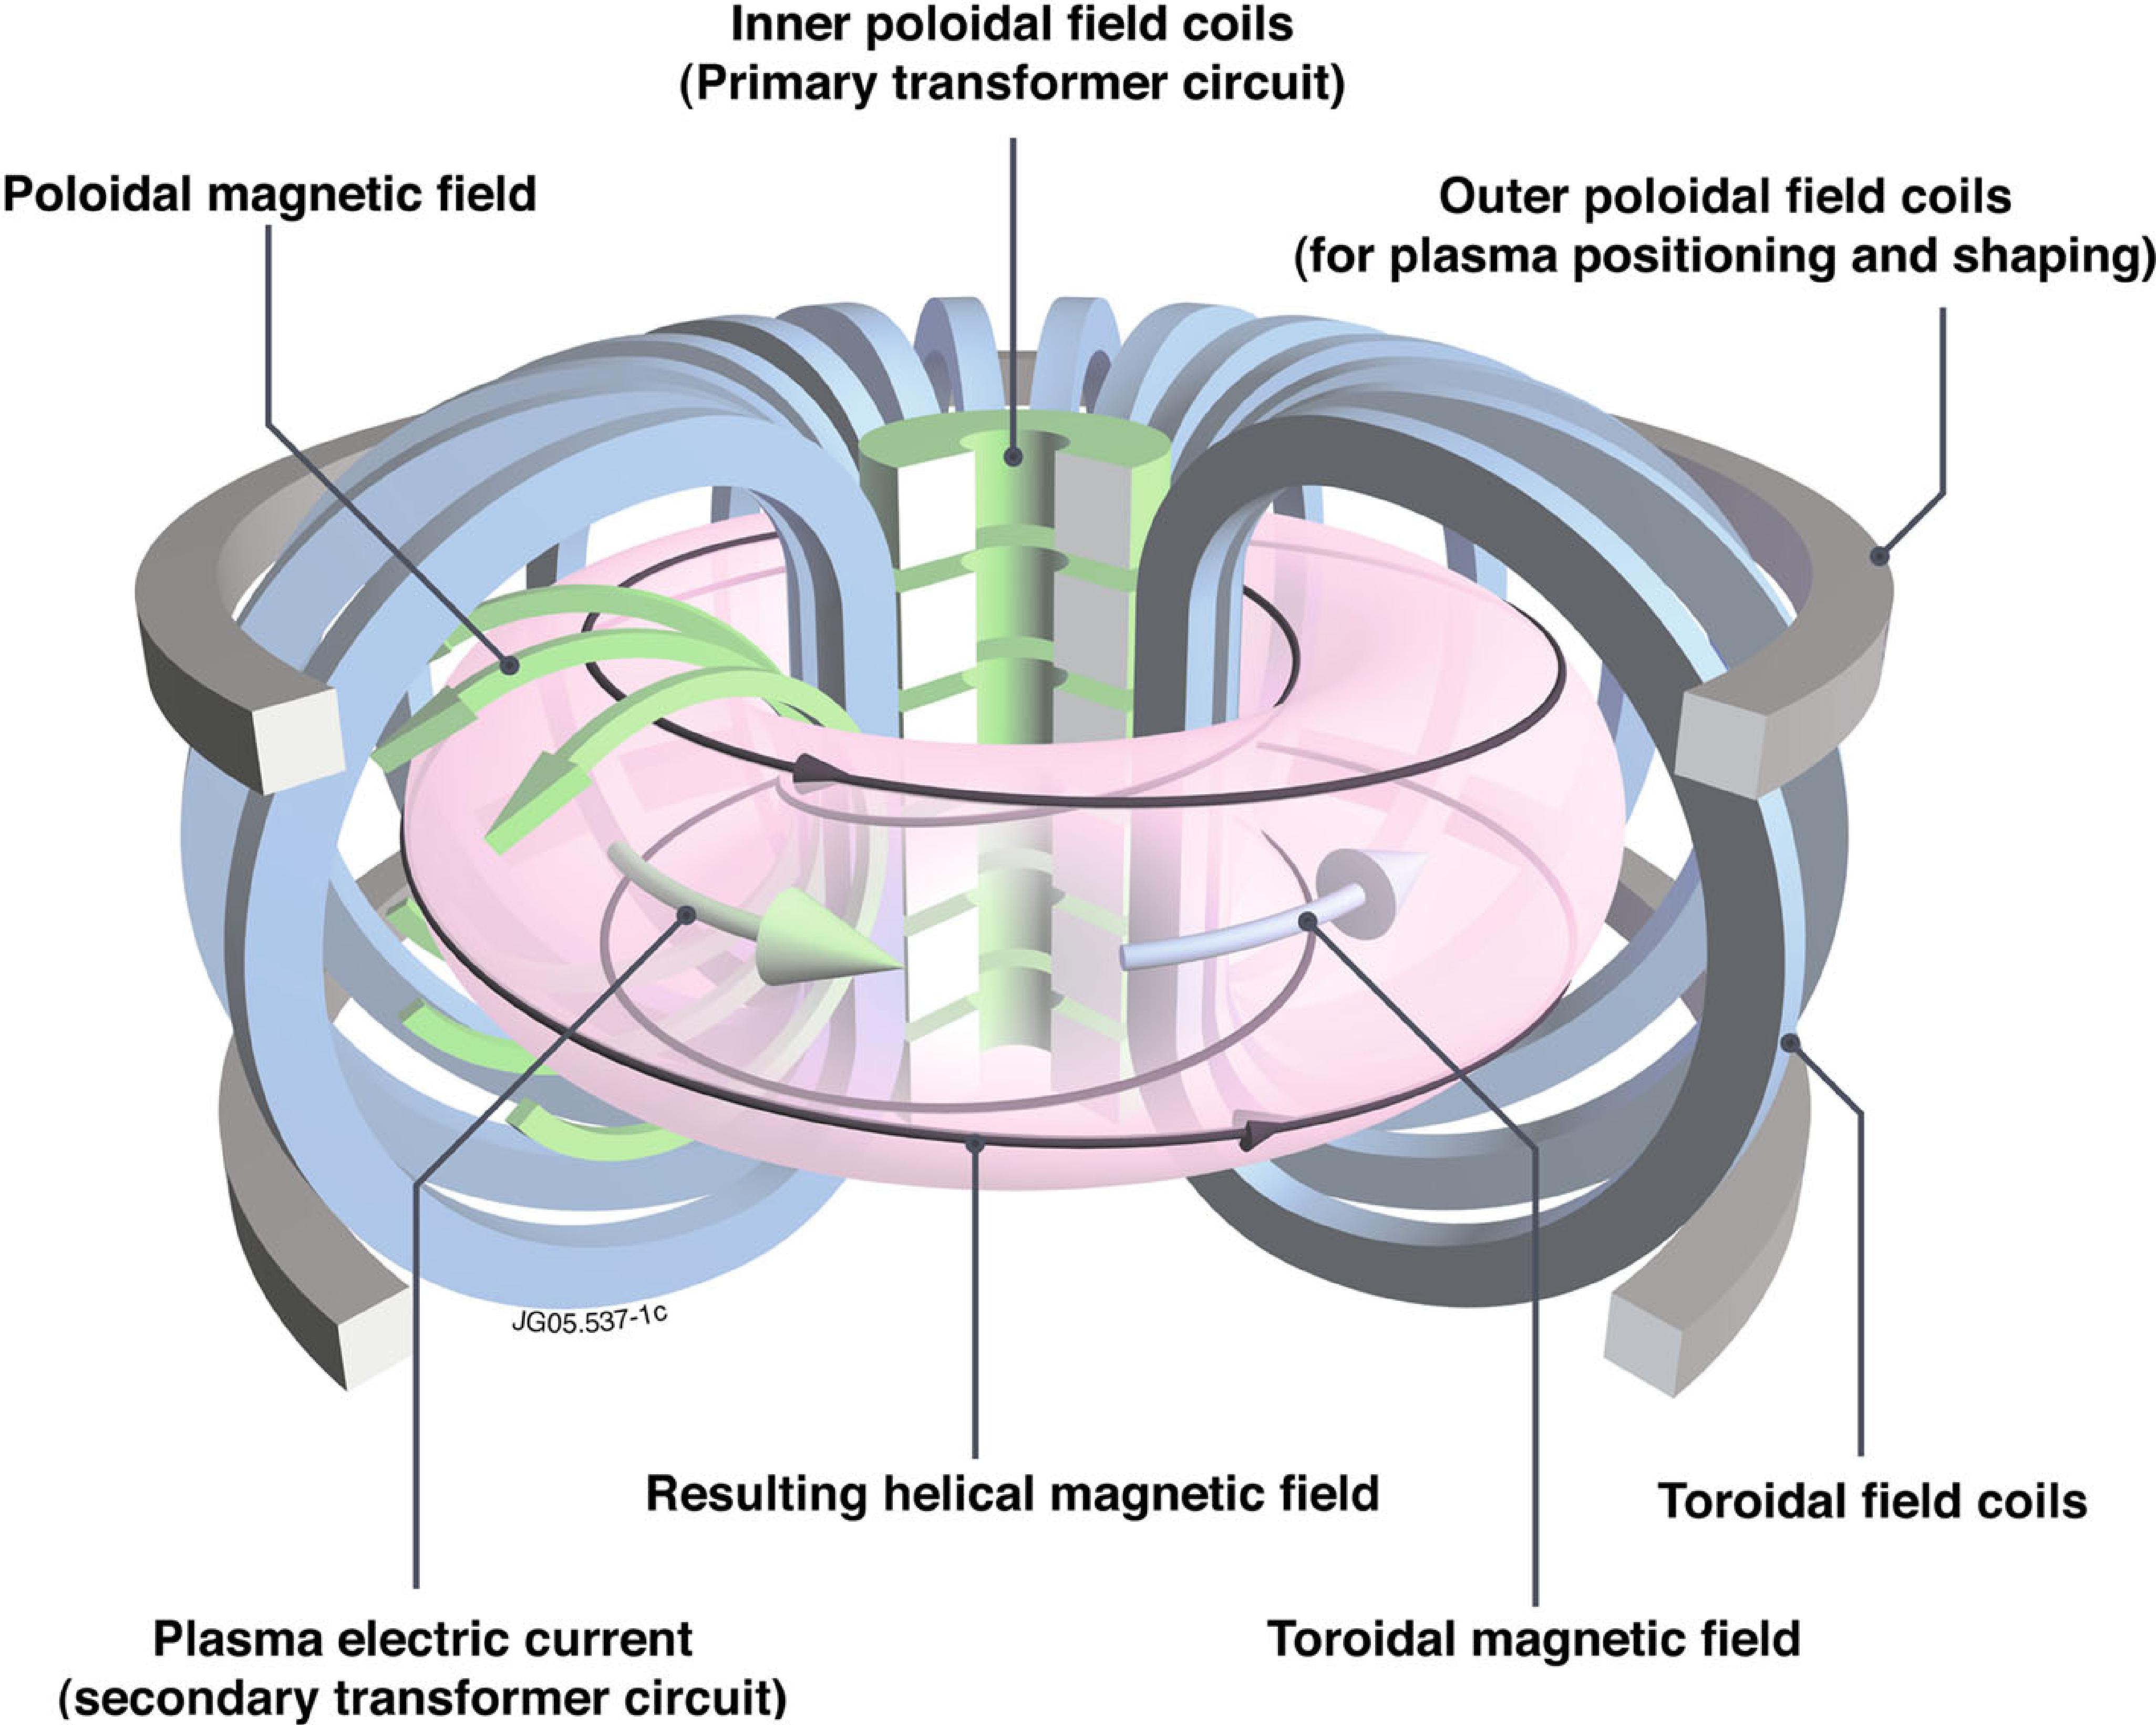
\includegraphics[width=1\linewidth]{./figures/tokamak.png}
        \caption{simplification of Tokamak device, the toroidal magnetic field is generated by the coils, and the poloidal magnetic field is generated by the plasma current amd the poloidal field coils. The plasma is heated up by several ways, and the fusion reaction can be sustained.}
        \label{}
    \end{figure}

    This confinement is realized by applying a strong magnetic field in the toroidal direction, The magnetic field is generated by a set of coils, which are arranged in a toroidal shape, and the plasma is heated by several ways (cite). The neoclassical geometries at stake in the tokamak leads to several physics phenomena such as charge separation in the tokamak, drifts cinematic and turbulences. The curvature and the gradient of magnetic field (cite) imposed by the geometry leads to $E \times B$ drift. Which impose to the tokamak a poloidal magnetic field component to counter this effect. This twist in the field line is called the safety factor and is defined as :
    $$q(\Psi) = \frac{1}{2\pi}\frac{\delta \chi (\Psi)}{\delta \Psi} \approx \frac{B_{tor}r}{B_{pol}R} \, ,$$
    With $\chi$ the toiridal magnetic flux. This safety factor is one of the most important measures in tokamak since the induced magnetic properties on the rational magnetic surface \footnote{Only rational value of the safety factor allows periodic field line} are of paramount importance for the confinement of the plasma. Indeed, we can define the shear stress as $\hat{s} = \frac{r}{q}\dv{q}{r},$ which measures how much the magnetic field line are twisted along the small radius of the tokamak. This shear explains why the turbulences grow on rational surfaces (no Landau Damping $k \centerdot B = 0$), and how they are damped into bigger scale flow (zonal flow) (cite).
    Indeed, the ra The consideration of the magnetic surfaces is also at the foreground for solving Ballonning equations in toiroidal geometry, since it will drive the definition of the toroidal functions of Ballonning modes, every discussed instabilities can be expressed using a toroidal geometry in the Ballooning space (cite). In addition to that the safety factor allows to have an insight of the strength of the current, which follows the $q$-profile (max in the center) (cite), this explains why the toroidal velocity of particle is lower on the edge than in the center, which allows some particle to be trapped in banana orbits.


    \section{Transports in Tokamak}
    Transports in tokamak are the main issue in the confinement of the plasma. Indeed, it allows perpendicular transport inside the tokamak, which leads to weakened confinement. Here we will study micro-instabilities, i.e small scale turbulences (gyro-bohm scaling), whose radial transport is really high. For these type of instabilities, the study is based on Kinetic Vlasov theory and not on MHD equations.
    Several types of micro-instabilities exists from \textbf{TEM} to \textbf{ITG} and \textbf{ETG} instabilities. The main goal of these instabilities is to transport the energy from the core of the plasma to the edge, where it can be evacuated, the largest transport in the TCV is due to the \textbf{TEM} mode. This mode is the results of the resonant interaction between trapped electron and Drift Wave (DW), it can be colisionless or dissipative.
    \subsection{Trapped particles and drifts}
    There is two type of cinematic for electrons in the plasma : run-away and trapped electrons. Majority if the electrons are runaway since to be trapped electrons must verify  : $v_\parallel \ll v_{th}$. However trapped electrons present a transit time much largerthan runaway, this leads to greater interaction with DW.
    These different of behavior regarding the DW leads to small scale instabilities.
    \subsubsection{Trapped particles}
    For a colisionless plasma $\lambda < eR$, with $\lambda$ the mean-free path, the main radial transport is caused by particle with low parallel velocity. Indeed, when the toroidal component of the magnetic field is much larger than the poloidal component, $\vert B_\Phi \vert \gg \vert B_{pol} \vert$ we have the simple $B$ relation for a torus $$B\propto \frac{1}{R-R_0} \, , $$ then in the $(r, \theta, z)$ coordinates we have  :
    $$B = B_0\left[1 - \frac{r}{R_0}\cos(\theta)\right]$$
    Hence, taking into account the toroidal drift we can derive the following equations using the guiding center equations (cite) :
    $$\dv{t}\left( r +\frac{m}{qB_p}v_\parallel\right) = 0 ,\, r - r_0 = -\frac{m}{qB_p}v_\parallel$$
    $r_0$ indicates the position of the turning point where the mirror effect occurs (cite). To be trapped the particle velocity should verify $v_\parallel \ll v_\perp$ more precisely from a simple energetic approach (cite) $$0 \leq v_\parallel \leq \sqrt{2\epsilon} v_\perp \,.$$ This partially explains why the velocity distribution of the electron (cite) is modified from a Boltzmann distribution to a more complex one, leading in a drop of conductivity (Spietzer condicivity). This also explain why the \textbf{TEM} disspitaive and colisionless are highly locallized in the trapped electron region. The banana shape formed as then the following width :
    $$\Delta r = \frac{m}{qB_p}v_\parallel \, $$

    This banana shape can be interpreted as a simple Lorentz force acting on the particle animated by a sufficiently high vertical drift motion.
    \begin{figure}[H]
        \centering
        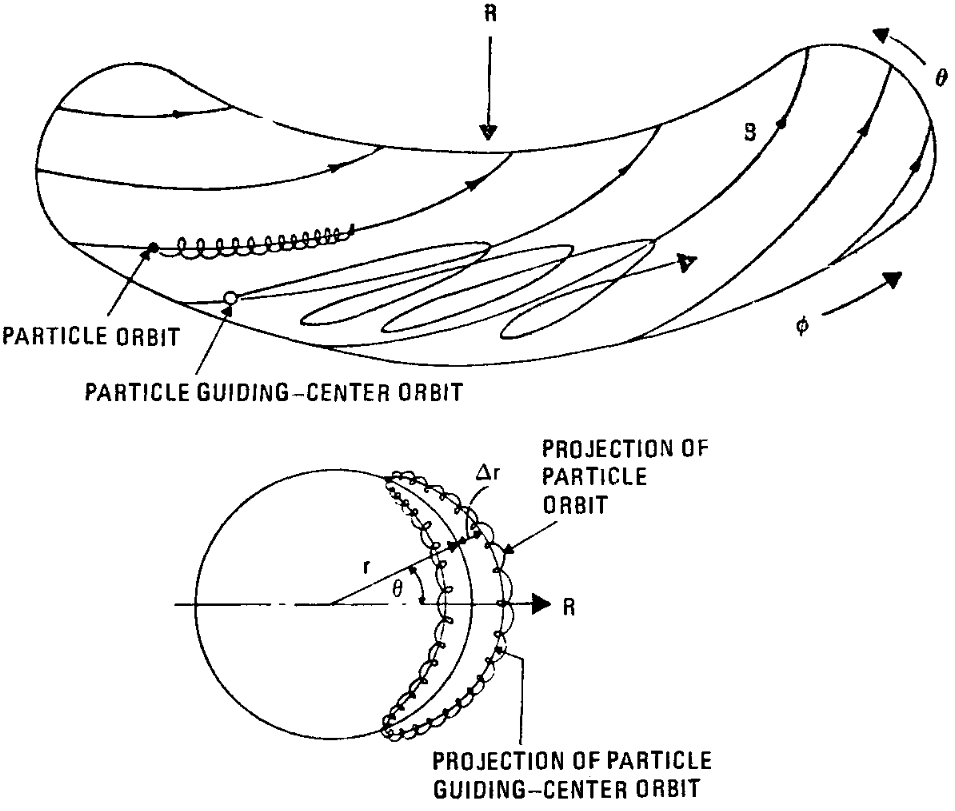
\includegraphics[width=1\linewidth]{./figures/banana.png}
        \caption{Trapped particle motion in the tokamak, the banana shape is due to the toroidal magnetic field, the particle is trapped in the magnetic well, and can interact with the DW. the second figure shows a cross section of the torus where we project the one banana orbit of the particle.}
        \label{}
    \end{figure}

    \subsubsection{Drift waves}
    Electron  DW instabilities that are at stakes here are governed by the famous \textbf{Hasegawa-Wakatani} equation due to non-adiabtic response of the electrons (the equilibrium is not reached after each oscillation of the wave) derived from a simple version of the drift kinetic equation from Vlasov theory. Hence, let's remind the general form of the general form of the H-W equation :
    \begin{equation}
        \begin{cases}
            \rho_s^2 \left(
            \dv{t} - v_0\nabla_\perp^2 \right) = D_\parallel\nabla_\parallel^2(\tilde{\Phi} - \frac{T\tilde{n}}{|e|n_0}) \\
            \frac{1}{n_0}\left(\dv{t} - D_0\nabla_\perp^2\right)\tilde{n} + \frac{v_r}{n_0}\partial_r\tilde{n_0} = D_\parallel\nabla_\parallel^2(\tilde{\Phi} - \frac{T\tilde{n}}{|e|n_0})
        \end{cases}\,.
    \end{equation}
    In the adiabtic limit, i.e when the particles diffuse faster than the wave, we can assume a simple a Boltzmann distribution of electrons with a small perturbation :
    $$\frac{\tilde{n}}{n} \approx \frac{\vert e \vert}{T} \tilde{\Phi} + \tilde{h}$$ this finally leads to the \textbf{Hasegawa-Mima} equation under the assumption : $ v_{thi} <\frac{w}{k_\parallel} \ll v_{the}$.
    \begin{equation}
        \begin{cases}
            \rho_s^2\dv{t}\nabla_\perp^2\tilde{\Phi} \approx \frac{1}{n_0}\left(\dv{\tilde{n}}{t} + \tilde{v_r\partial_r n_0}\right) \\
            \partial_t \frac{\vert e \vert \tilde{\Phi}}{T} + \partial_t \tilde{h} - \rho_s^2\dv{t}\nabla_\perp^2\tilde{Phi}  + v^{*}\partial_y\frac{\vert e \vert \tilde{\Phi}}{T} = 0
        \end{cases}
    \end{equation}
    This leads to the following dispersion relation for the drift waves with $w_r$ the real frequency of the wave and $\gamma$ the growth rate (the imaginary part of the frequency) :
    $$\omega_r = \frac{w_{*}}{1 + k_\perp^2\rho_s^2}, \quad \frac{\gamma}{w_r} = \pi \frac{w_r - w_{*}}{k_\parallel v_{e,th}}$$

    We can denote $\frac{w-w_*}{k_\perp^2v_{e,th}}$ the non-Boltzmann factor for electron DW. The reader will note that this study is independant of trapped electron, this is why in order of magnitude the growth rate is quite low, however when we increase the transit time of electron (by trapping),
    we can show (cite), that the non-Boltzmann factor is increasing, leading to a higher growth rate, notably because of the introduction of $w_{D,e}$ the electron curvature drift frequency. Indeed, for colisionless trapped electron mode the non-Boltzmann factor is given by : $\frac{w - w_*}{w_{e,D}}e^{-R/L_n}\sqrt{\frac{R}{L_n}}$ which is definitively larger than the electron DW non-Boltzmann correction factor.
    leading to the following growth rate : $$\frac{\gamma}{w_r} = i \pi \frac{w - w_*}{w_{e,D}}e^{-R/L_n}\sqrt{\frac{R}{L_n}},$$ explaining why \textbf{CTEM} are much more unstable than classical electron DW. Explaining also why the main instabilities are located in the banana region where the coherence time of the electrons are much more larger, same conclusions can be driven from the Dissipative Trapped electron mode. (cite). This instabilities leads to inverse cascade of energy (\emph{Kolmogorov}), leading to interaction with large scale flow (zonal flow) (cite).
\end{multicols}

\begin{figure}[H]
    \centering
    \includegraphics[width=1\linewidth]{./figures/balloning_TEM.png}
    \caption{Cross section view - On the left we have the fourier Ballonning mode $n = 6$, characteric from the TEM mode, it presents characteristic odahsdoisahd oiashd oiahsdoiashdo iashd oiasdh osaih doasi dhosa ihoioias doihsa doisah doisah doiash dosaihd osaihd. On the right we have a simulated TEM mode, with the same shape characteric in a positive shear flow oasihd oasdh osaidh osahi oasidh osaidh oasdh oasidh ohasdoihsado isahoid asoid , from anannana and ananannanaaa}
    \label{}
\end{figure}
\begin{multicols}{2}
    \subsection{Radial Transport}
    These micro-instabilities are one of the best candidates to explain high radial transport, indeed as we saw previously the resonating trapped electron allows a high fluctuation in the density field and in the magnetic pressure. The radial transport is allowed by the non-adiabatic componment of the electron response, indeed if we calculate the radial flux due to \textbf{CTEM} we obtained :
    $$\langle\tilde{v_r}\tilde{n} \rangle = -\sum_{k}\langle\tilde{v_r}\rangle_k^2\frac{\Delta w_k}{w_*^2} \nabla \langle n \rangle - D_{res} \nabla \langle n \rangle $$
    The coupling between the resonant diffusion coefficient $D_{res}$ plays an important role in the corrugation of the density profile, in the radial direction, the diffusion coefficient is established by the following :

    This radial dependency is the only density dependency retained for the following part. We already explained why this radial transport can be an issue for high confinement, butr one can also highlight that it can also stabilize the plasma, this is why it is of first importance to study these density profile fluctuations.
    \section{Wave propagation in plasma}
    \subsection{Plasma as a medium}
    To study the density profile, many diagnostics methods exists ,like Doppler Reflectometry, RCDR, Short pulse reflectometry \dots The study here will be based on the Short Pulse Reflectometry (\textbf{SPR}), this methdod consists in probing the magnetized plasma with short Pulse (<ns) microwaves operating in the time domain at a fixed frequency under normal incidence with respect to the cut-off surface and the variation of the delay of the reflected pulses. The probing signal, is sensitive to density variation since it will change the cut-off position, this is why it can
    be used to have deeper insights of the turbulences characteristics
    \subsection{Wave equation}
    Assuming a monochromatic electromagnetic-wave and using the Maxwell equations, we can derive the local complex dieletric tensor, and the considerated wave wave equation :

    \begin{equation}
        \begin{rcases}
            \laplacian E -  \vec{\nabla}\nabla \cdot E = -\frac{\omega^2}{c^2} \hat{\epsilon} E \\
            \hat{\epsilon}_{ik} = \delta _{ik} - \frac{4\pi i}{\omega} \sigma_{ik}
        \end{rcases}
    \end{equation}
    with $\sigma_{ik}$ the conductivity tensor. To establish this equation multiple assumption have been made, linear Ohm's law is applicable, cold plasma (cite), neglect chaotic motion of the particles, which implies neglecting the kinetic effect. To simplify the problem we will assume the plasma to be stationnarym and neglecvt all kind of damping. Then in a carthesian coordinates system with $z$ axis driven by a constant magnetic field,
    $\vec{B} = B_0\vec{e}_z$, we can derive the following dielectric tensor
    $$\hat{\epsilon} = \begin{pmatrix}
            1 - \frac{\omega_p^2}{\omega^2} & i\frac{\omega_c}{\omega}        & 0 \\
            -i\frac{\omega_c}{\omega}       & 1 - \frac{\omega_p^2}{\omega^2} & 0 \\
            0                               & 0                               & 1
        \end{pmatrix}$$
    With : $\epsilon = 1 - \frac{\omega_{pe}^2}{\omega^2 - w_{ce}^2}$, $g = \frac{w_{ce}w_{pe}^2}{w(w^2 9 W_{ce}^2)} - \frac{w_{ci}w_{pi}^2}{w(w^2 9 W_{ci}^2)}$;
    $ \eta  = 1 - \frac{w_{pe}^2}{w^2} -  \frac{w_{pi}^2}{w^2}; \quad w_{pi} = \sqrt{\frac{4\pi n e^2}{m_i}}; \quad w_{ci} = \frac{eH}{m_i c}$

    $w_{pi}$ stands for the electron or plasma frequency and $w_{ci}$ is the cyclotron frequency for the i species. We will consider the electron component preponderant in the next study since we are dealing with microwave frequency. The wave equation can be simplified to the following :

    \begin{equation}
        \begin{rcases}
            (S_{yz} - \epsilon)E_x - igE_y - \Pi_{xy}E_z = 0 \\
            (S_{zx} - \epsilon)E_x + igE_x - \Pi_{yz}E_z = 0 \\
            (S_{xy} - \eta)E_z -\Pi_{xz}E_x - \Pi_{yz}E_y = 0
        \end{rcases}
    \end{equation}
    Defining : $S_{ij} = N_i^2 + N_j^2; \quad \Pi_{ij} = N_iN_j ; \quad N_{i} = \frac{k_iw}{c}$
    For the \textbf{SPR} study the wave is perpendicular to the external magnetic field, hence we can simplify the system to the following :
    \begin{equation}
        \begin{rcases}
            (N_y^2 - \epsilon)E_x - igE_y = 0 \\
            (N_x^2 - \epsilon)E_y + igE_x = 0 \\
            (S_{xy} - \eta)E_z = 0
        \end{rcases}
    \end{equation}

    Which leads to two different types of solution respectively the ordinary mode ($\mathcal{O}$) and the extraordinary mode ($\mathcal{X}$).
    \setlength{\tabcolsep}{18pt}
    \renewcommand{\arraystretch}{1.5}
    \begin{center}
        \begin{tabular}{|| c  | c||}
            \hline
            $\mathcal{O}$       & $\mathcal{X}$                       \\
            \hline\hline
            $S_{xy} - \eta = 0$ & $(N_y^2 - \epsilon)E_x - igE_y = 0$ \\
            $E_y = 0$           & $(N_x^2 - \epsilon)E_y + igE_x = 0$ \\
            $E_x = 0$           & $E_z = 0$                           \\
            \hline
        \end{tabular}
    \end{center}
    The $\mathcal{O}$ mode corresponds to the mode with electric field parallel to the external magnetic field, hence the propagation does not depend on this latter but only on the density profile. The $\mathcal{X}$ mode is the mode with electric field perpendicular to the external magnetic field, hence the propagation depends on the magnetic field and the density profile. The dispersion relation of the wave can be derived locally from the wave equation, and we can obtain :
    $$k^2 = \frac{w^2}{c^2} \eta \approx \frac{w^2}{c^2}\left(1 - \frac{n}{n_c}\right); \quad n_c = \frac{m_ew}{4 \pi e^2} $$
    Here we can see that the wave number vanish at $n = n_c$, this is the cut-off layer where the wave is reflected.
    The k-spectrum of the $\mathcal{X}$ is much more complicated and include plasma resonances where thermal effects must be taken into account. For this study we will limit ourself to the $\mathcal{O}$ mode. Then from solving the Helmotz equation (local dependancy of the wave number) $$\pdv{E_z}{x} + k(x)E_z = 0$$ and appying the \textbf{WKB} approximation (slow variation of the plasma parameters) we can derive from the perturbation method the following equation (cite):
    $$ \laplacian E_z  + \frac{w^2}{c^2}\left(1 - \frac{n_0(x)}{n_c}\right)E^1_z =  \frac{w^2}{c^2}\left(\frac{\delta n(x,y)}{n_c}\right)E^0_z $$
    This shows at least that the amplitude of the scattered probing wave is dependent of the turbyulence amplitude and turbulence spectra, this is why probing the plasma with such electromagnetic wave can be useful for retrieving all kinds of data from the plasma. From this, other kind of probing method can be imagnied such as Doppler reflectometry where the incident wave has a given angle, to scan the correlation length of the turbulences \dots.
\end{multicols}

\begin{figure}[H]
    \centering
    \includegraphics[width=1\linewidth]{./figures/field_SPR.pdf}
    \label{}
\end{figure}
\captionof{figure}{\textbf{SPR} setup using the \emph{O.Krutkin and A.combette \textbf{LEONARDO} simulations from the \textbf{CUWA} code}, the probing wave is sent to the plasma, and the reflected wave from the cut-off is measured, the delay between the two waves is a measure of the plasma density profile, in addition to the pulse shape that has been altered by the turbulenences (eq). Here we plot the contours of the density profile, with cold density perturbations (black contour lines on the left plot), the probing wave is reflected by the cut-off layer (initial probing wave on the left and after a $\Delta t \approx 10 ns$ we got the reflected scattered wave on the right). The third plot on the right shows the density profile width its perturbations (filled), a liner density profile $$n(x,y) = \frac{x}{L} \left(n_c + \delta n(x,y)\right).$$ as been chosen accoriding to (cite). The curvature of the grid has been set to the $R = 0.25m$ to mimic the TCV geometry.}
\begin{multicols}{2}
    \chapter{Linear Regime Study}
    The goal of this study is to find a way to link the plasma density perturbations to the reflected pulse characterics. First we will study a simple 1 dimensional model proposed by (\emph{Oleg Krutkin}) applied in a given range of turbulence amplitude and size and then we will extend this study to a morte general 2D model using the \textbf{CUWA} code.
    \section{1 dimensional study}
    Assuming a simple plasma density profile $n(x)$, we can study the wave propagation in the plasma. The goal of this approach is to find a way to link the plasma density perturbations to the reflected pulse delay. To retrieve some information about the pulse delay we will
    use a statistical approach to get rid of the randomness implies by the perturbations considerations.
    The delay of the probing wave is given by the following formula  : $$\tau_c = 2 \int_0^L \frac{dx}{v_g}$$ Where $v_g$ is the group velocity of the wave, $L$ is the position of the cut-off.
    From the simple assumption $\langle \delta n \rangle = 0 $ for an Ordinary mode the  $v_g$ expression obtained [] can be used to expand the integral to the following :
    $$\frac{2}{c} \int_0^L \frac{dx}{\sqrt{1 - \frac{x}{L} - \frac{\delta n }{n_c}}}$$ The main contribution of this integral comes from the vicinity of the cut-off layer, Where the group velocity is the smallest.
    We can discuss the relevance of this expansion this the main contribution of the integral comes from the cut-off region where the WKB approximation cannot be applied.

    \subsection{Perturbed Density Profile}
    \subsubsection{General perturbation profile}
    First let's consider to simplify a gaussian perturbation density profile (we will see later that the spectrum of the vector number is not a gaussian but a non trivial power spectrum due to the two type of energy cascade). From this, the considered integral can be writen in the following way :

    $$\tau_d = \frac{2}{c} \int_0^L \frac{dx}{\sqrt{1 - \frac{x}{L} - \frac{\delta n\exp(-\frac{(x - L)^2}{8l_{cx}^2})}{n_c}}}$$

    This integral is not trivial to solve in from an anlytical way, which is necessary to exhibit the possible statistical features of the dealay. This is why we can suggest developing a first order perturbation profile which leads to step like perturbations.

    \subsubsection{Step-like perturbation}
    \paragraph{Model}

    With a step-size perturbation characterized by $l_{cx}$ length. This allows to get an analytical expression of the integral for different density profile. However, to get this simplification, we need to assume that the perturbation is small enough such that the WKB approximation can be applied.
    This is the case for the linear regime, where the perturbation is small enough such that the cut-off layer is not too much perturbed (i.e $\delta_x \ll l_{cx}$). In the case of a large perturbation, an other step perturbation localized far from the cut-off layer can be used to get the same result, which breaks the main assumption of this approach (see fig.1).
    It's relatively trivial to obtain the following expression for the delay [cite Krutkin] :
    $$\tau_d = \frac{4L}{c} - \frac{2L}{c}\sqrt{\frac{L}{l_{cx}}}\frac{\delta n}{n_c} $$
    To test this assumption we can compare the analytical expression with the numerical integration of the wave equation, for numerous gaussian perturbations with characteristics length $l_{cx}$ and amplitude $\delta n$. The results are shown in the figure \ref{fig:delay_amp_norm_2}. Some discrepancies are observed for large perturbations, but the analytical expression seems to be a good approximation for small perturbations, except for tiny one [cite]. However, One have to introduce a correction
    factor to the analytical expression to get a better agreement with the numerical integration. This $l_{cx}$ dependant factor is given has not been studied yep but it highlights the linitations of current 1D model \footnote{The integration of the gaussian integral was also tackled, with a second order bell-approximation, leading to logarithmic dependancies over the plasma parameters, however the formula was to complicated to exhibits the statistical properties of the delay refers to appendix}.

    \paragraph{statistical approach}
    The statistical approach is to consider the perturbation as a random variable, and to compute the statistical properties of delay of the probing wave. This approach is relevant for the linear regime, where the perturbation is small enough such that the cut-off layer is not too much perturbed (i.e $\delta_x \ll l_{cx}$). Foe example we can compute the standard deviation of the delay depending on the standard deviation of perturbations.
    This gives us the following :
    $$\sigma_{\tau_d} = \frac{2L}{c}\sqrt{\frac{L}{l_{cx}}}\frac{\sigma_{\delta n}}{n_c}$$
\end{multicols}

\begin{figure}[H]
    \centering
    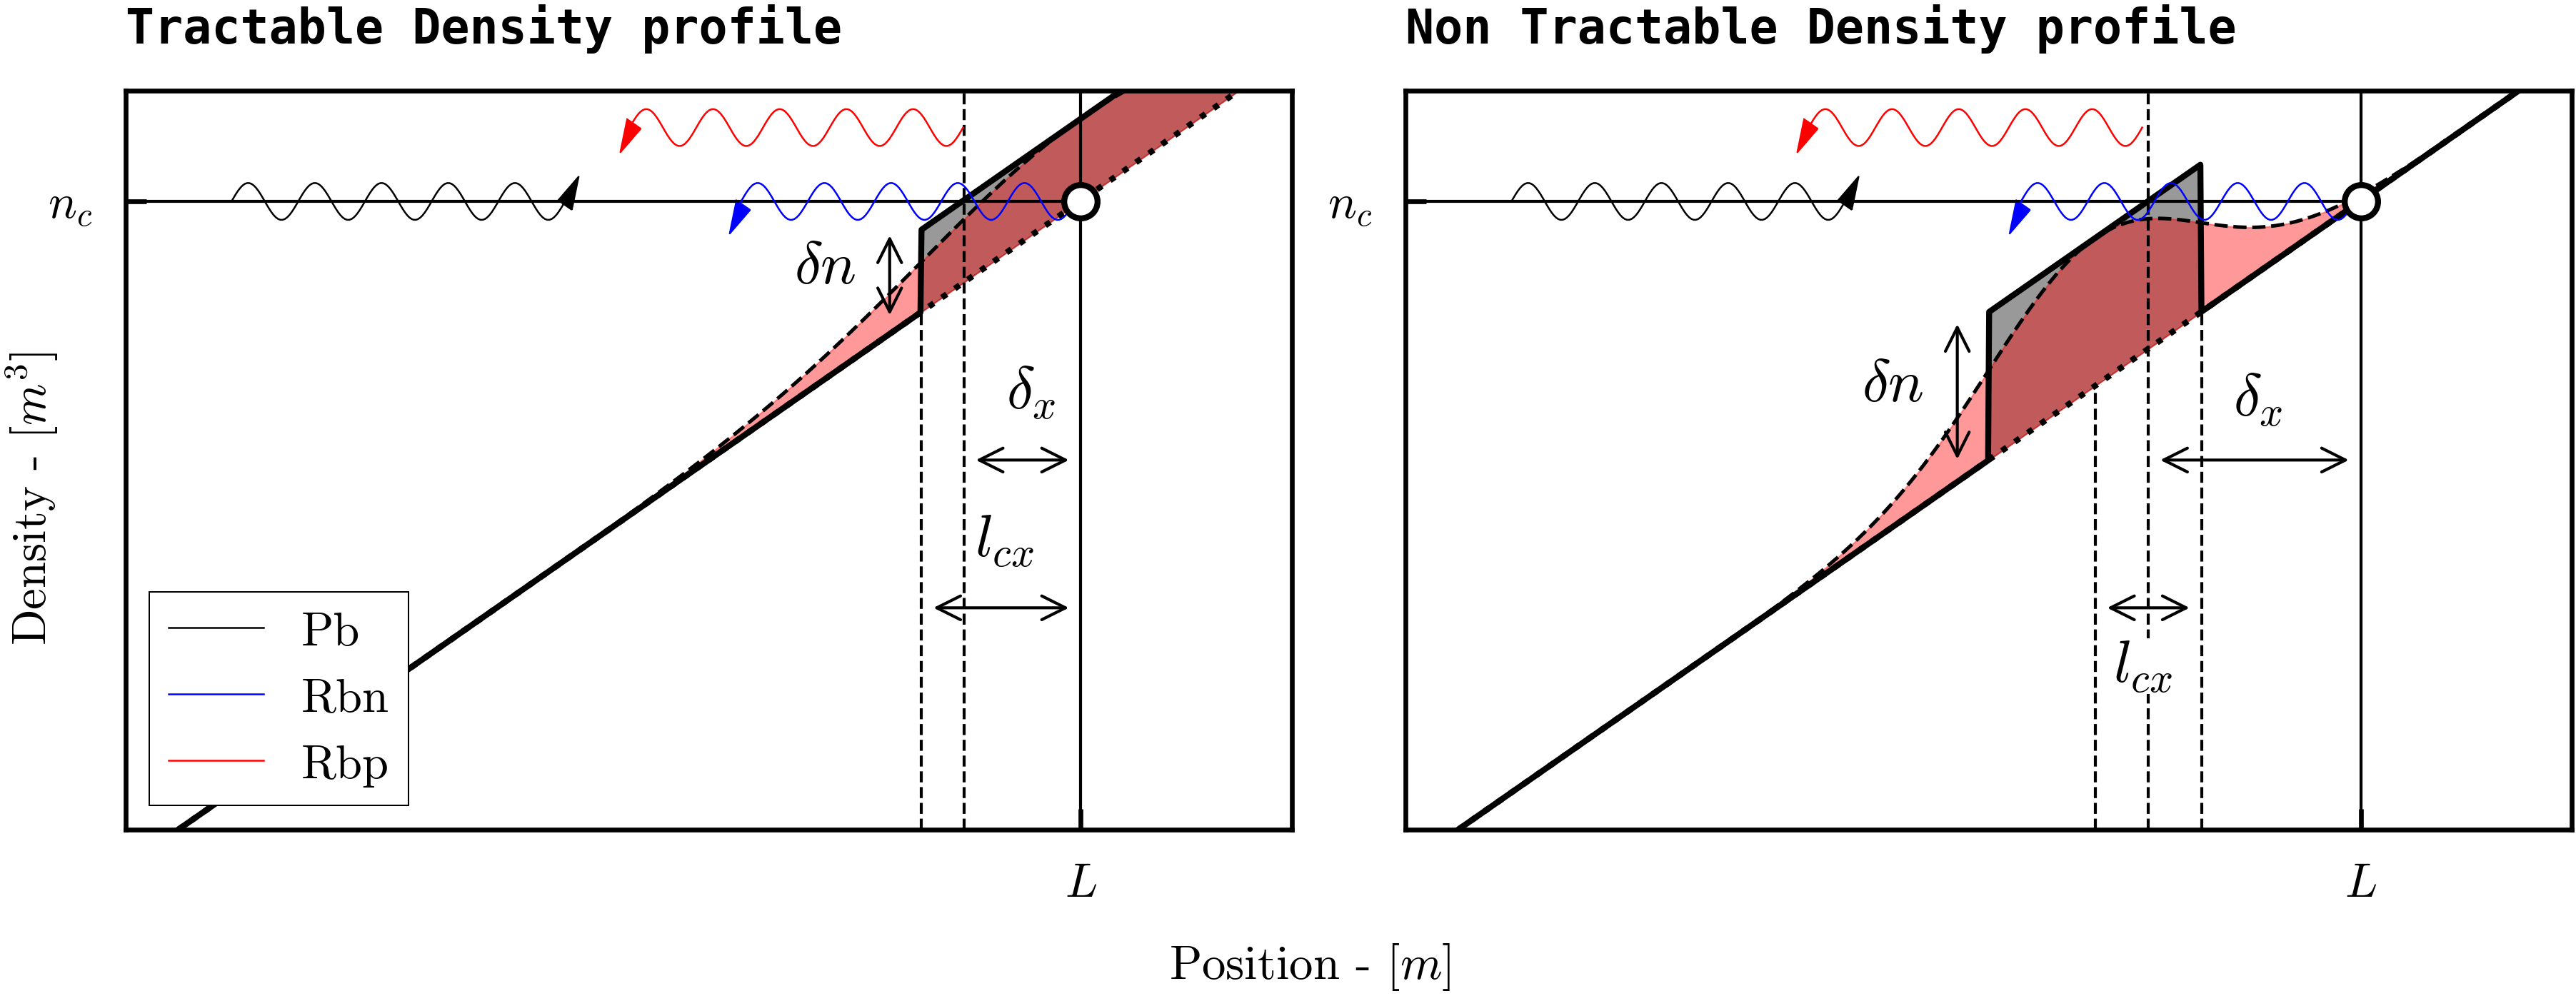
\includegraphics[width = 1\linewidth]{./figures/density_profile.png}
    \caption{Here we plot the density profile of the plasma for different perturbation amplitude, in grey the step-like model perturbation and in coral the gaussian one. For large value density perturbation, the model leads to a contradiction with its assumption, given by a small cut-off layer shift.
        The gaussian perturbation seems to be a better approach for large perturbation. The blue Pb wave is the probing wave, red Rbp wave is the reflected one and blue Rbn wave is the normal reflected wave, in absence of perturbation.}
    \label{}
\end{figure}
\begin{multicols}{2}

    \section{2 dimensional study}
    The 1D model is a good approximation for small perturbations, but it has some limitations for large perturbations. The 2D model is a more realistic approach, but it is more difficult to solve. The main difficulty comes from the fact that the wave equation is a partial differential equation, and the perturbation density profile is not separable. However, the 2D model can be solved numerically using the finite difference method. The main goal of this approach is to find a way to link the plasma density perturbations to the reflected pulse delay. To retrieve some information about the pulse delay we will use a statistical approach to get rid of the randomness implies by the perturbations considerations.
    \subsection{Numerical Integration for plasma density}
    Kinetic model for plasma, equations \dots
    \subsection{Full wave Modelling}
    CUWA CODE : Finite difference method, wave equation, plasma density, \dots
    \subsection{Background profiles}
    \begin{itemize}
        \item For the linear background profile, the global density profile will be the following :
              $$n(x,y) = n_c \frac{x}{L} + \delta n(x,y).$$ WIth $\delta n $ the 2D gaussian turbulence profile
        \item For the quadratic background profile L, stands for the gradient scale at the cut-off. Here we choose the following formula to get the value of 1 of the gradient at L, which gives us :
              $$n(x,y) = n_c \left[1.25 - \frac{(1.5L_0 - x)^2}{L_0^2} \right] + \delta n (x,y)$$
        \item One can remark that for small $x$ the turbulence profile is getting preponderant, especially for high amplitudes turbulences, this non realistic behaviour can be
              tackled using a linear dependence in the amplitude of the turbulences. $$n(x,y) = \frac{x}{L}\left( n_c  + \delta n \right)$$
    \end{itemize}

    \begin{figure}[H]
        \centering
        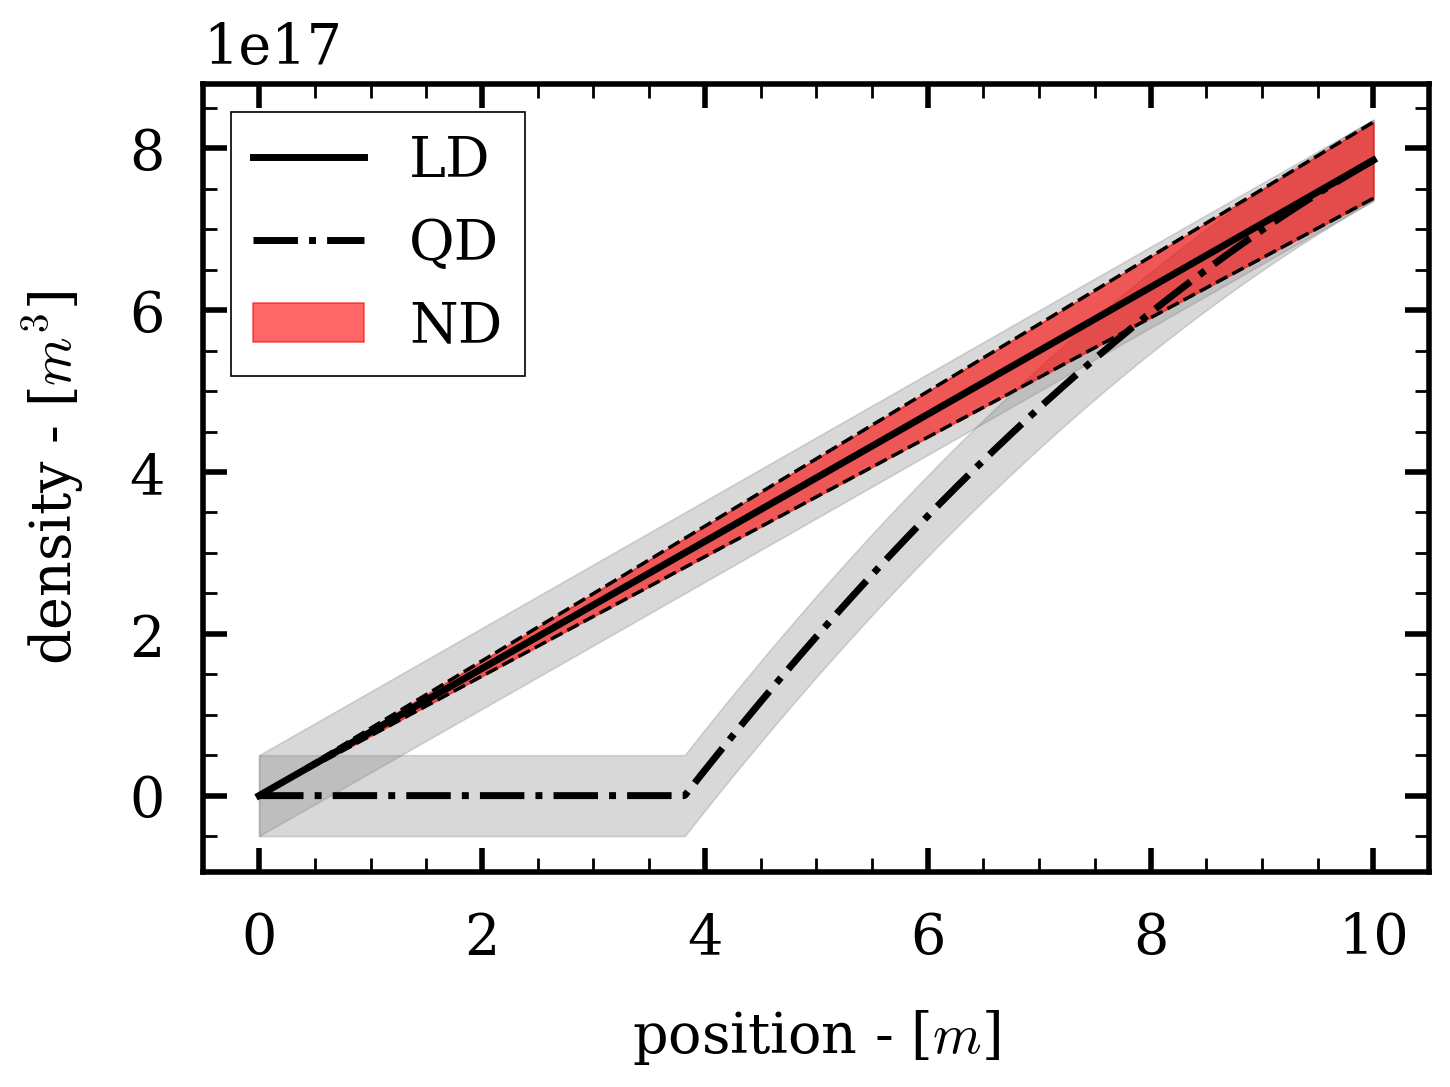
\includegraphics[width=1\linewidth]{./figures/background_density.png}
        \caption{Here we plot the three density profile with filled deviation range, in order to see the effect of the linear amplitude dependence of turbulences. \textbf{LD} stands for the linear density profile in the following, \textbf{QD} for the quadratic one, and \textbf{ND} for the linearized turbulence profile}
        \label{fig:barrier}
    \end{figure}
    \section{Numerical Integration}
    For both 1D and 2D model we can compare the delay rms obtained by integrations, and see if a simple analytical integration of the 1D model can be realistic, which should help releasing some computations time. For the other statistical properties of the delay and the pulse shape, we should limit ourselves to the 2D approach.
    Which is computationally more expensive, but more realistic. The integration has been done for several background profiles to see if they have strong influence on the probing wave propgation.
    \subsection{statistical Properties of the delay}

\end{multicols}

\begin{figure}[H]
    \centering
    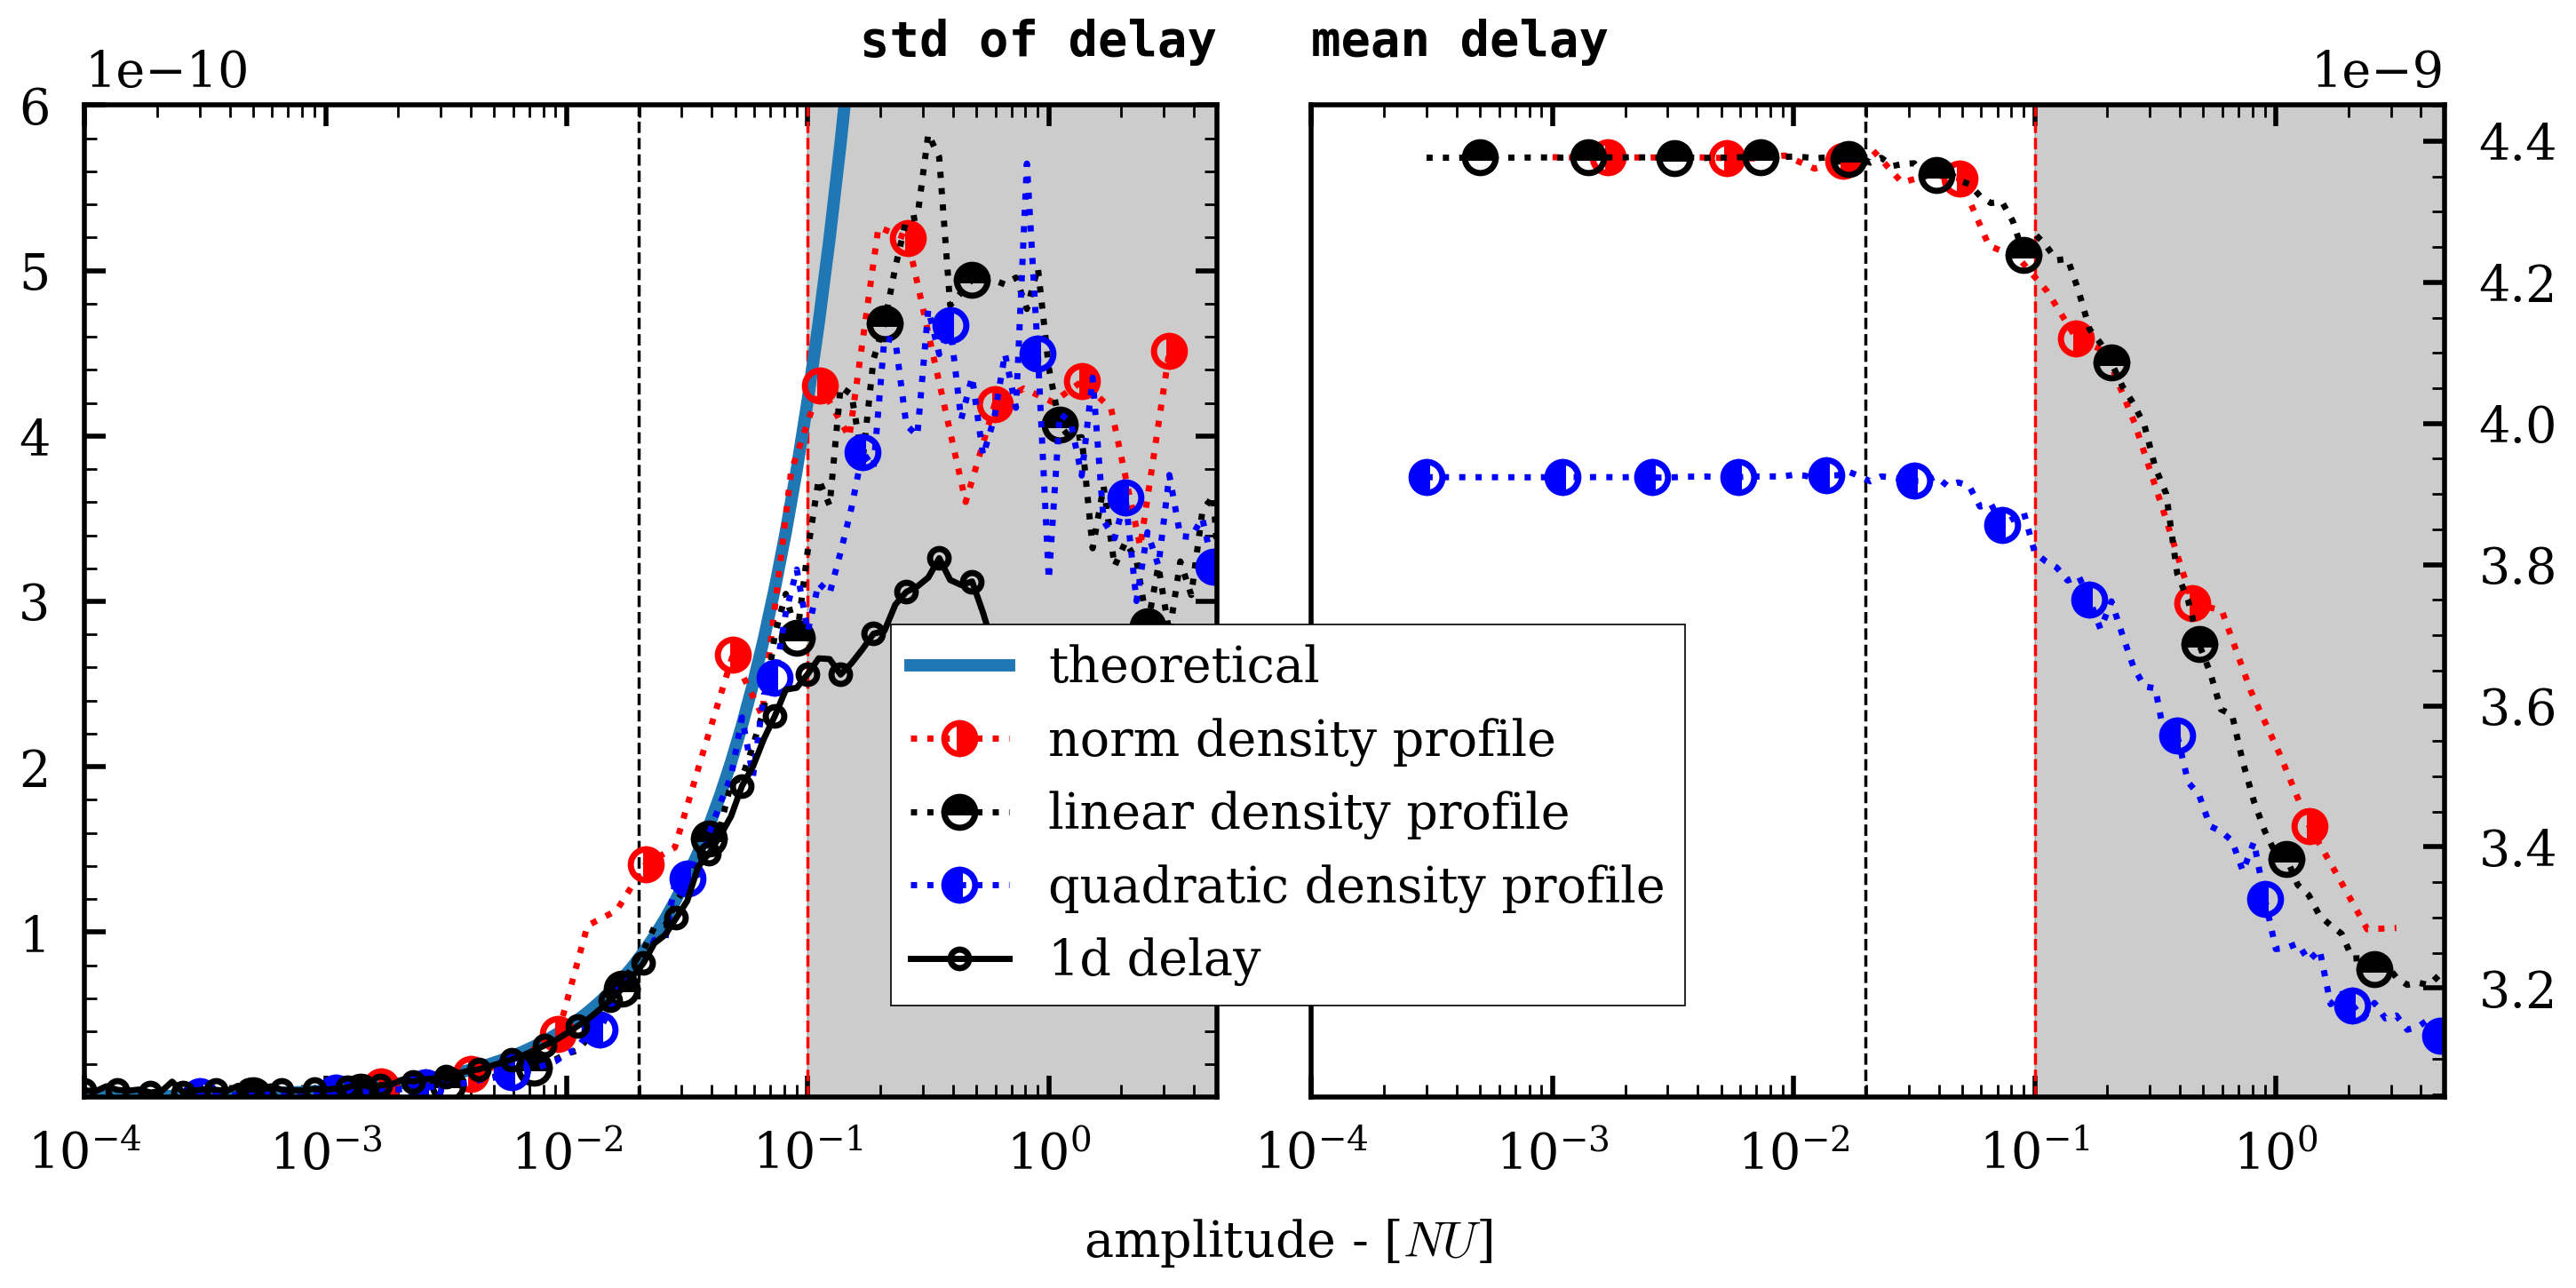
\includegraphics[width=1\linewidth]{./figures/delay_amp_norm_2.png}
    \caption{Respectively standard deviation of the delay and mean delay evolution. The red vertical line stands for the first critical value unearthed by [], the black one is the second critical value. For both parameter,
        the analytical expression seems to be a good approximation for small perturbations. For perturbations larger than the first critical value the model collapses has intended, and this for every background profile. We can also note that even if the deviation of the delay has an erratic behavior after the first critical value, the mean delay decrease smooothly.
        This is strongly related to the displacement of the cut-off layer, indeed the wave is reflected much more quickly due to the presence of strong perturbations.}
    \label{fig:barrier}
\end{figure}
\begin{multicols}{2}
    \subsection{Pulse shape Study}
    The pulse shape is also an interesting parameter to study, indeed it can give us some information about the plasma density profile, since the pulse shape can be modified by the presence of perturbations due to multiple scattering effects and dispersive effects [see O mode dispersion relation].
    The dependance of the pulse shape over the background density profile will be also studied with linear, quadratic and linear modified perturbation profile.


    One can expect to have a much larger and randomness dependent pulse, at high turbulence amplitude due to multiple scattering.
    Indeed the reflected pulse will be a superposition of all scattered pulse, which should be characterized by a growing tail of the pulse distribution in delay and in width. This can be seen in the figure \ref{fig:barrier}.This will be observed on the mean pulse shape, and on the mean statistical parameters of the pulse shape.
    \begin{figure}[H]
        \centering
        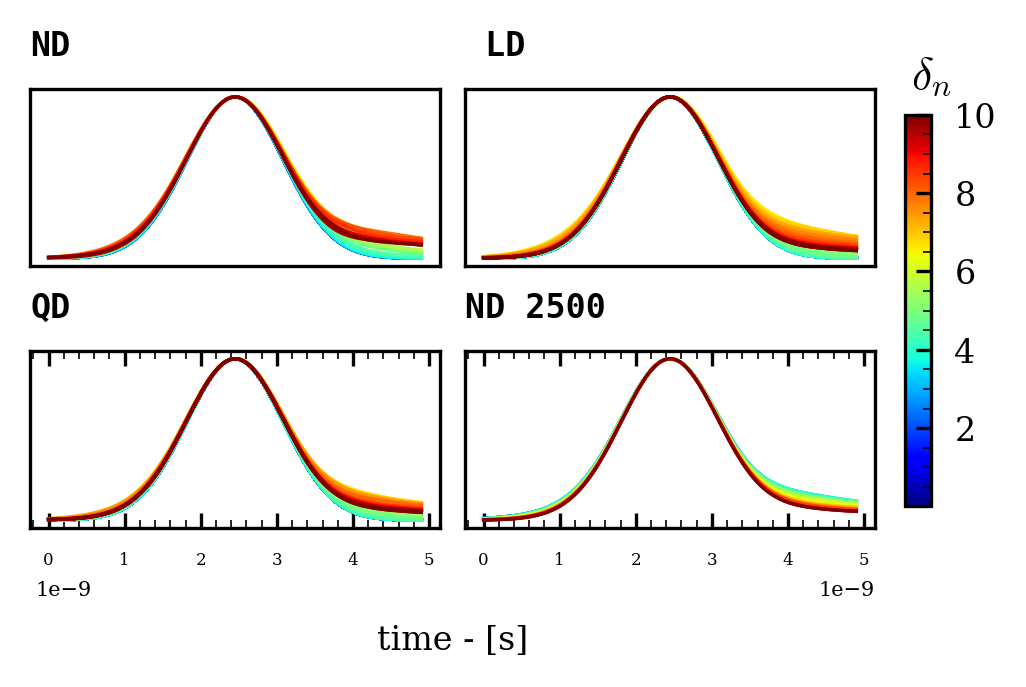
\includegraphics[width=1\linewidth]{./figures/pulse_shape.png}
        \label{fig:barrier}
    \end{figure}
    \captionof{figure}{For all density profile, the pulse shape is getting broader and broader for large perturbations, and the delay is getting larger and larger. This is due to the presence of multiple scattering, and dispersive effects. This will be characterized further by the study of the mean skewness of the pulse shape.}
    One way to vizualize that is plotting the distribution of some parameters of the pulse shape for different perturbation amplitude.
    Here we choose to study the rms and the amplitude of the pulse, Indeed, it allows to the beahavior of the pulse width and height during the linear-non linear transition.
    This is showm in the following figure. This type of plots are called violins plot, where filled zone stands for the distribution of the random variable, calculate over every samples.

\end{multicols}
\begin{figure}[H]
    \centering
    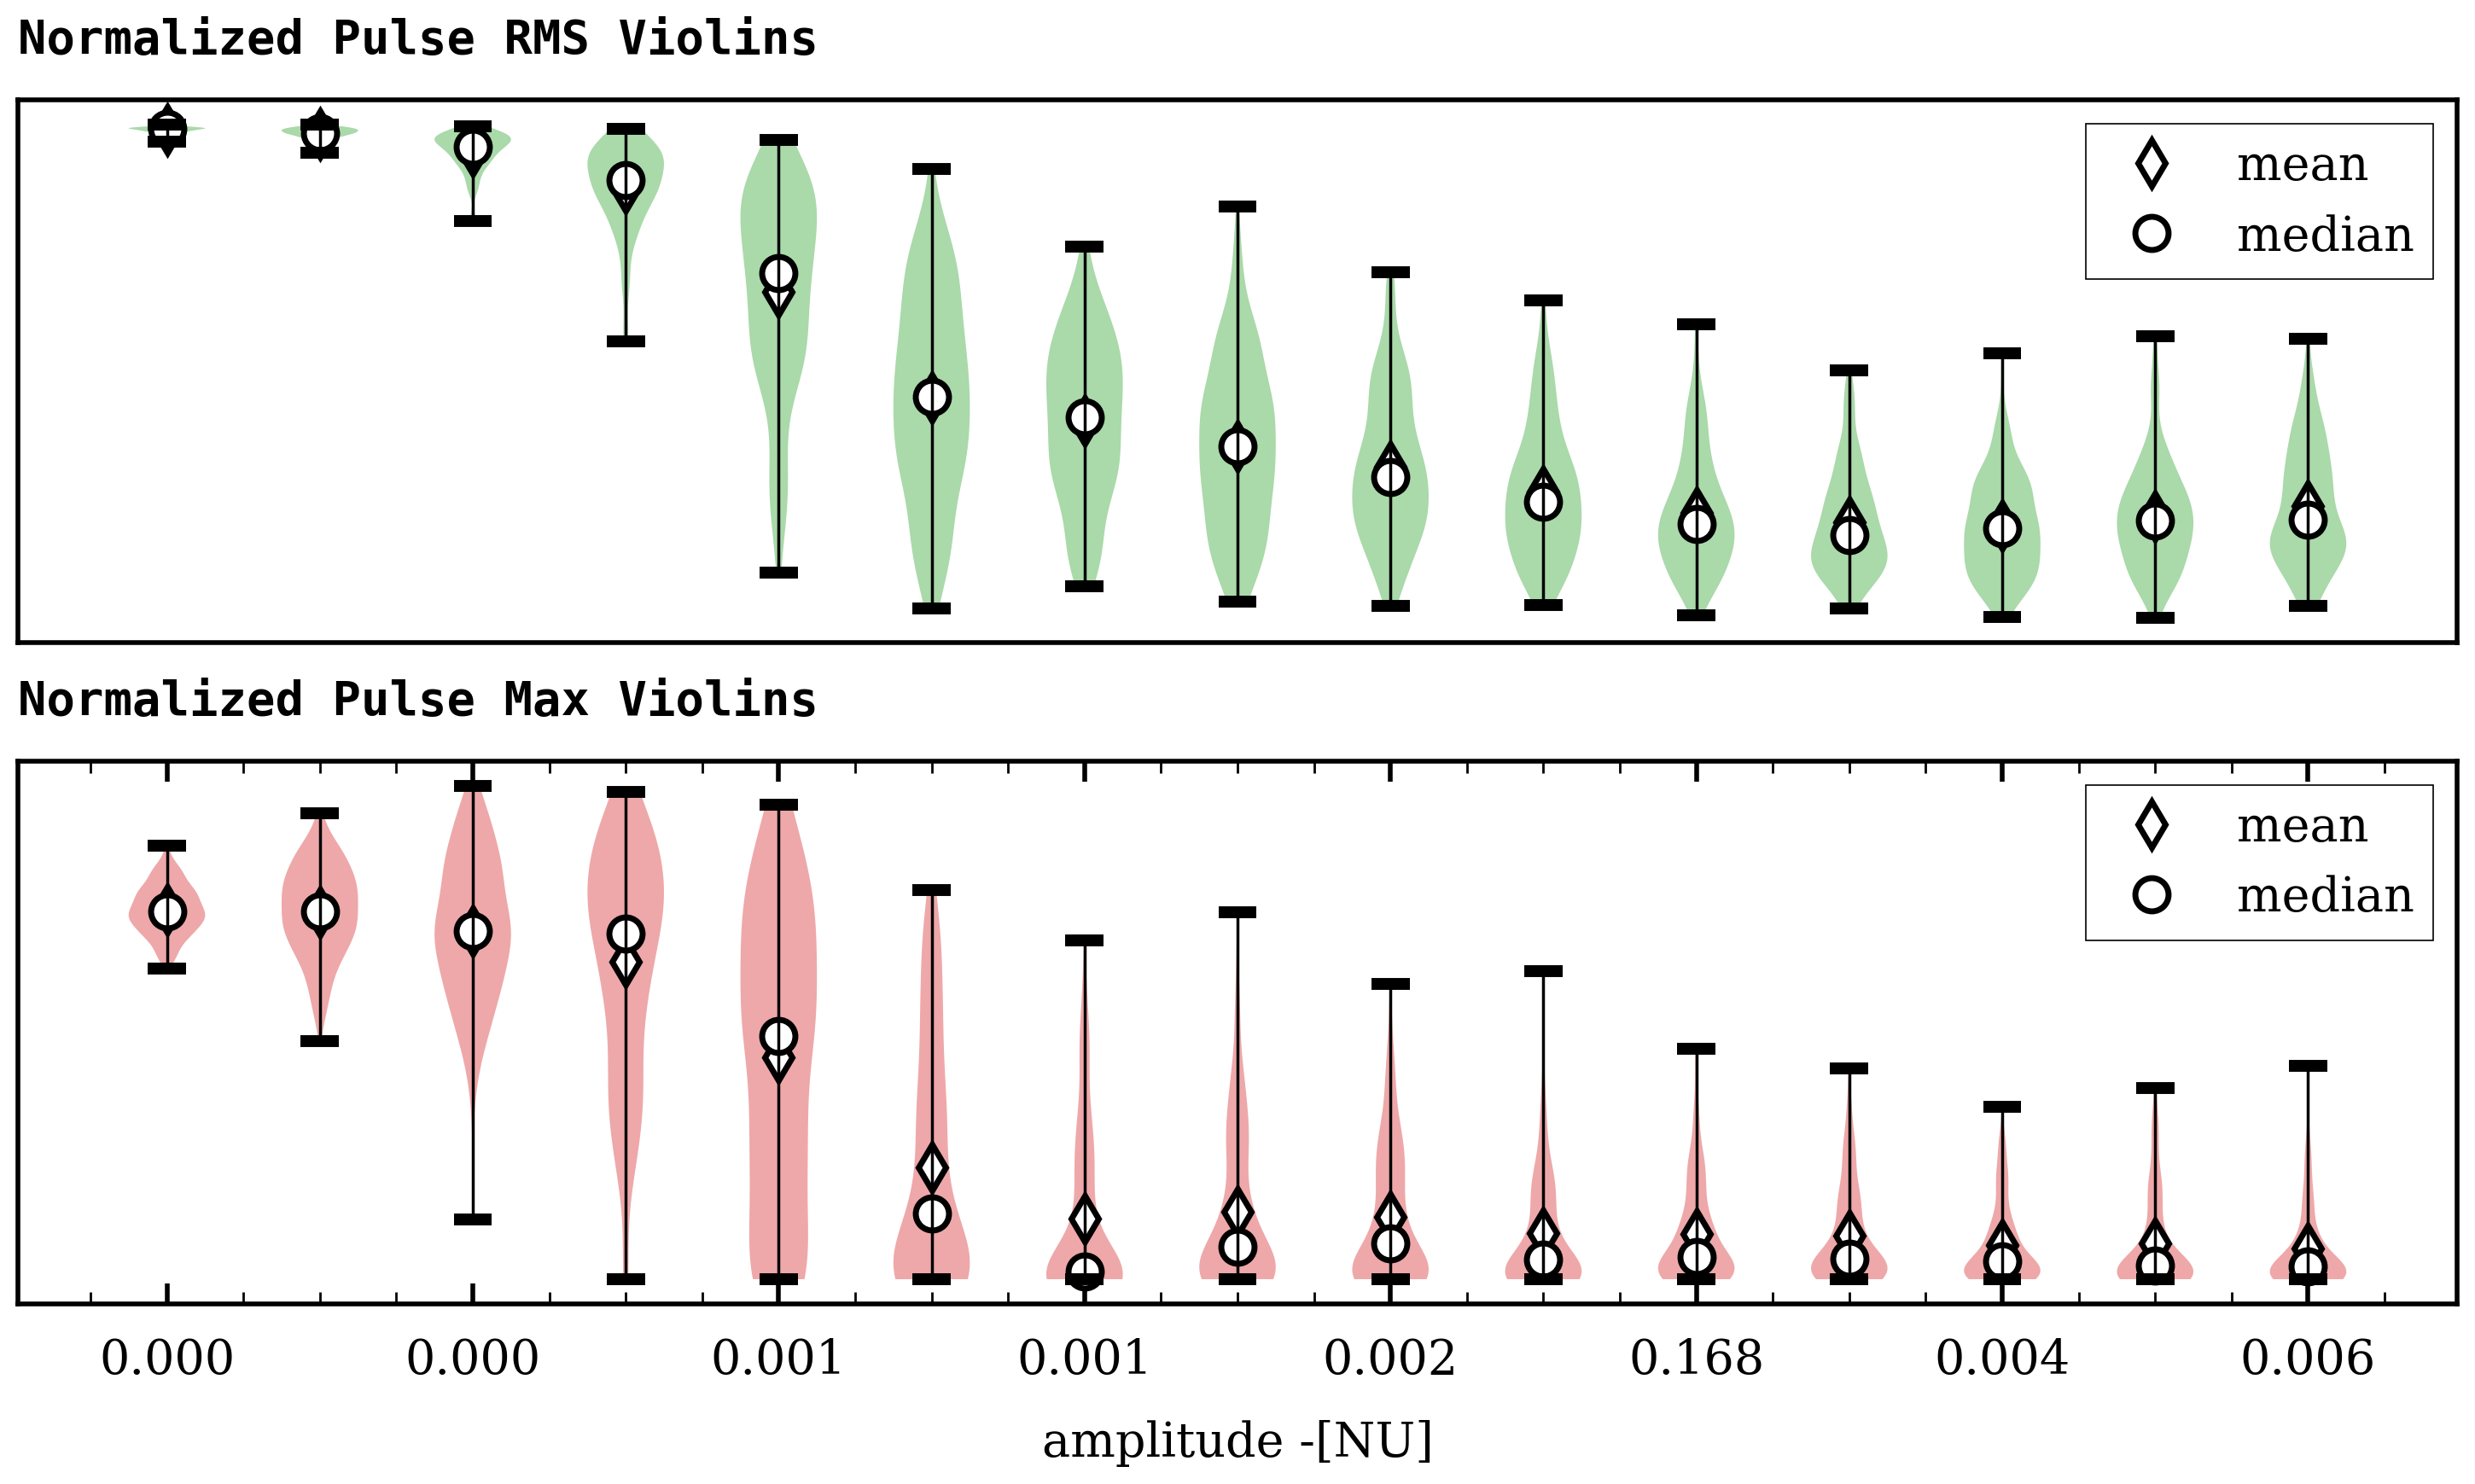
\includegraphics[width=1\linewidth]{./figures/pulse_overview.png}
    \caption{Here we plot the distribution of the pulse rms and amplitude for different perturbation amplitude, for the linear profile background profile \textbf{LD}. The distribution of the pulse rms  and amplutude is getting broader and broader during the transition regime, this is due to randomness introduced by the perturbations, which seems to remains at large amplitudes, even if the distribution is getting quite constant.
        Lets also note that the mean of both distribution is getting smaller due to presence of multiple scattering, reaching a plateau at high turbulence ampliude.}
    \label{fig:barrier}
\end{figure}
\begin{multicols*}{2}
    The characteristic turbulence amplitude scale for the pulse shape transition seems to be the first critical value with $\delta n \approx 1e^{-3}$. Thanks to this study, we can unearth a way of characterizing the transition regime, using the pulse shape for multiple background profiles. For deeper insights about the pulse transition regime, we can study the skewness of the pulse shape, which should give us more information about the "broader and broader" distrubution of the pulse shape.
    Note that we are talking about the transition regime of the pulse shape, since the transition regime regarding the delay seems to appear at much larger amplitude at the second critical value $\delta n \approx 1e^3$ ax shown in Fig.2.3.

    One important question we have to solve is the following, which metrics is the most relevant to characterize the transition regime. This will help us, to build a relevant datasets to tackle the non linear regime.

\end{multicols*}
\begin{figure}[H]
    \centering
    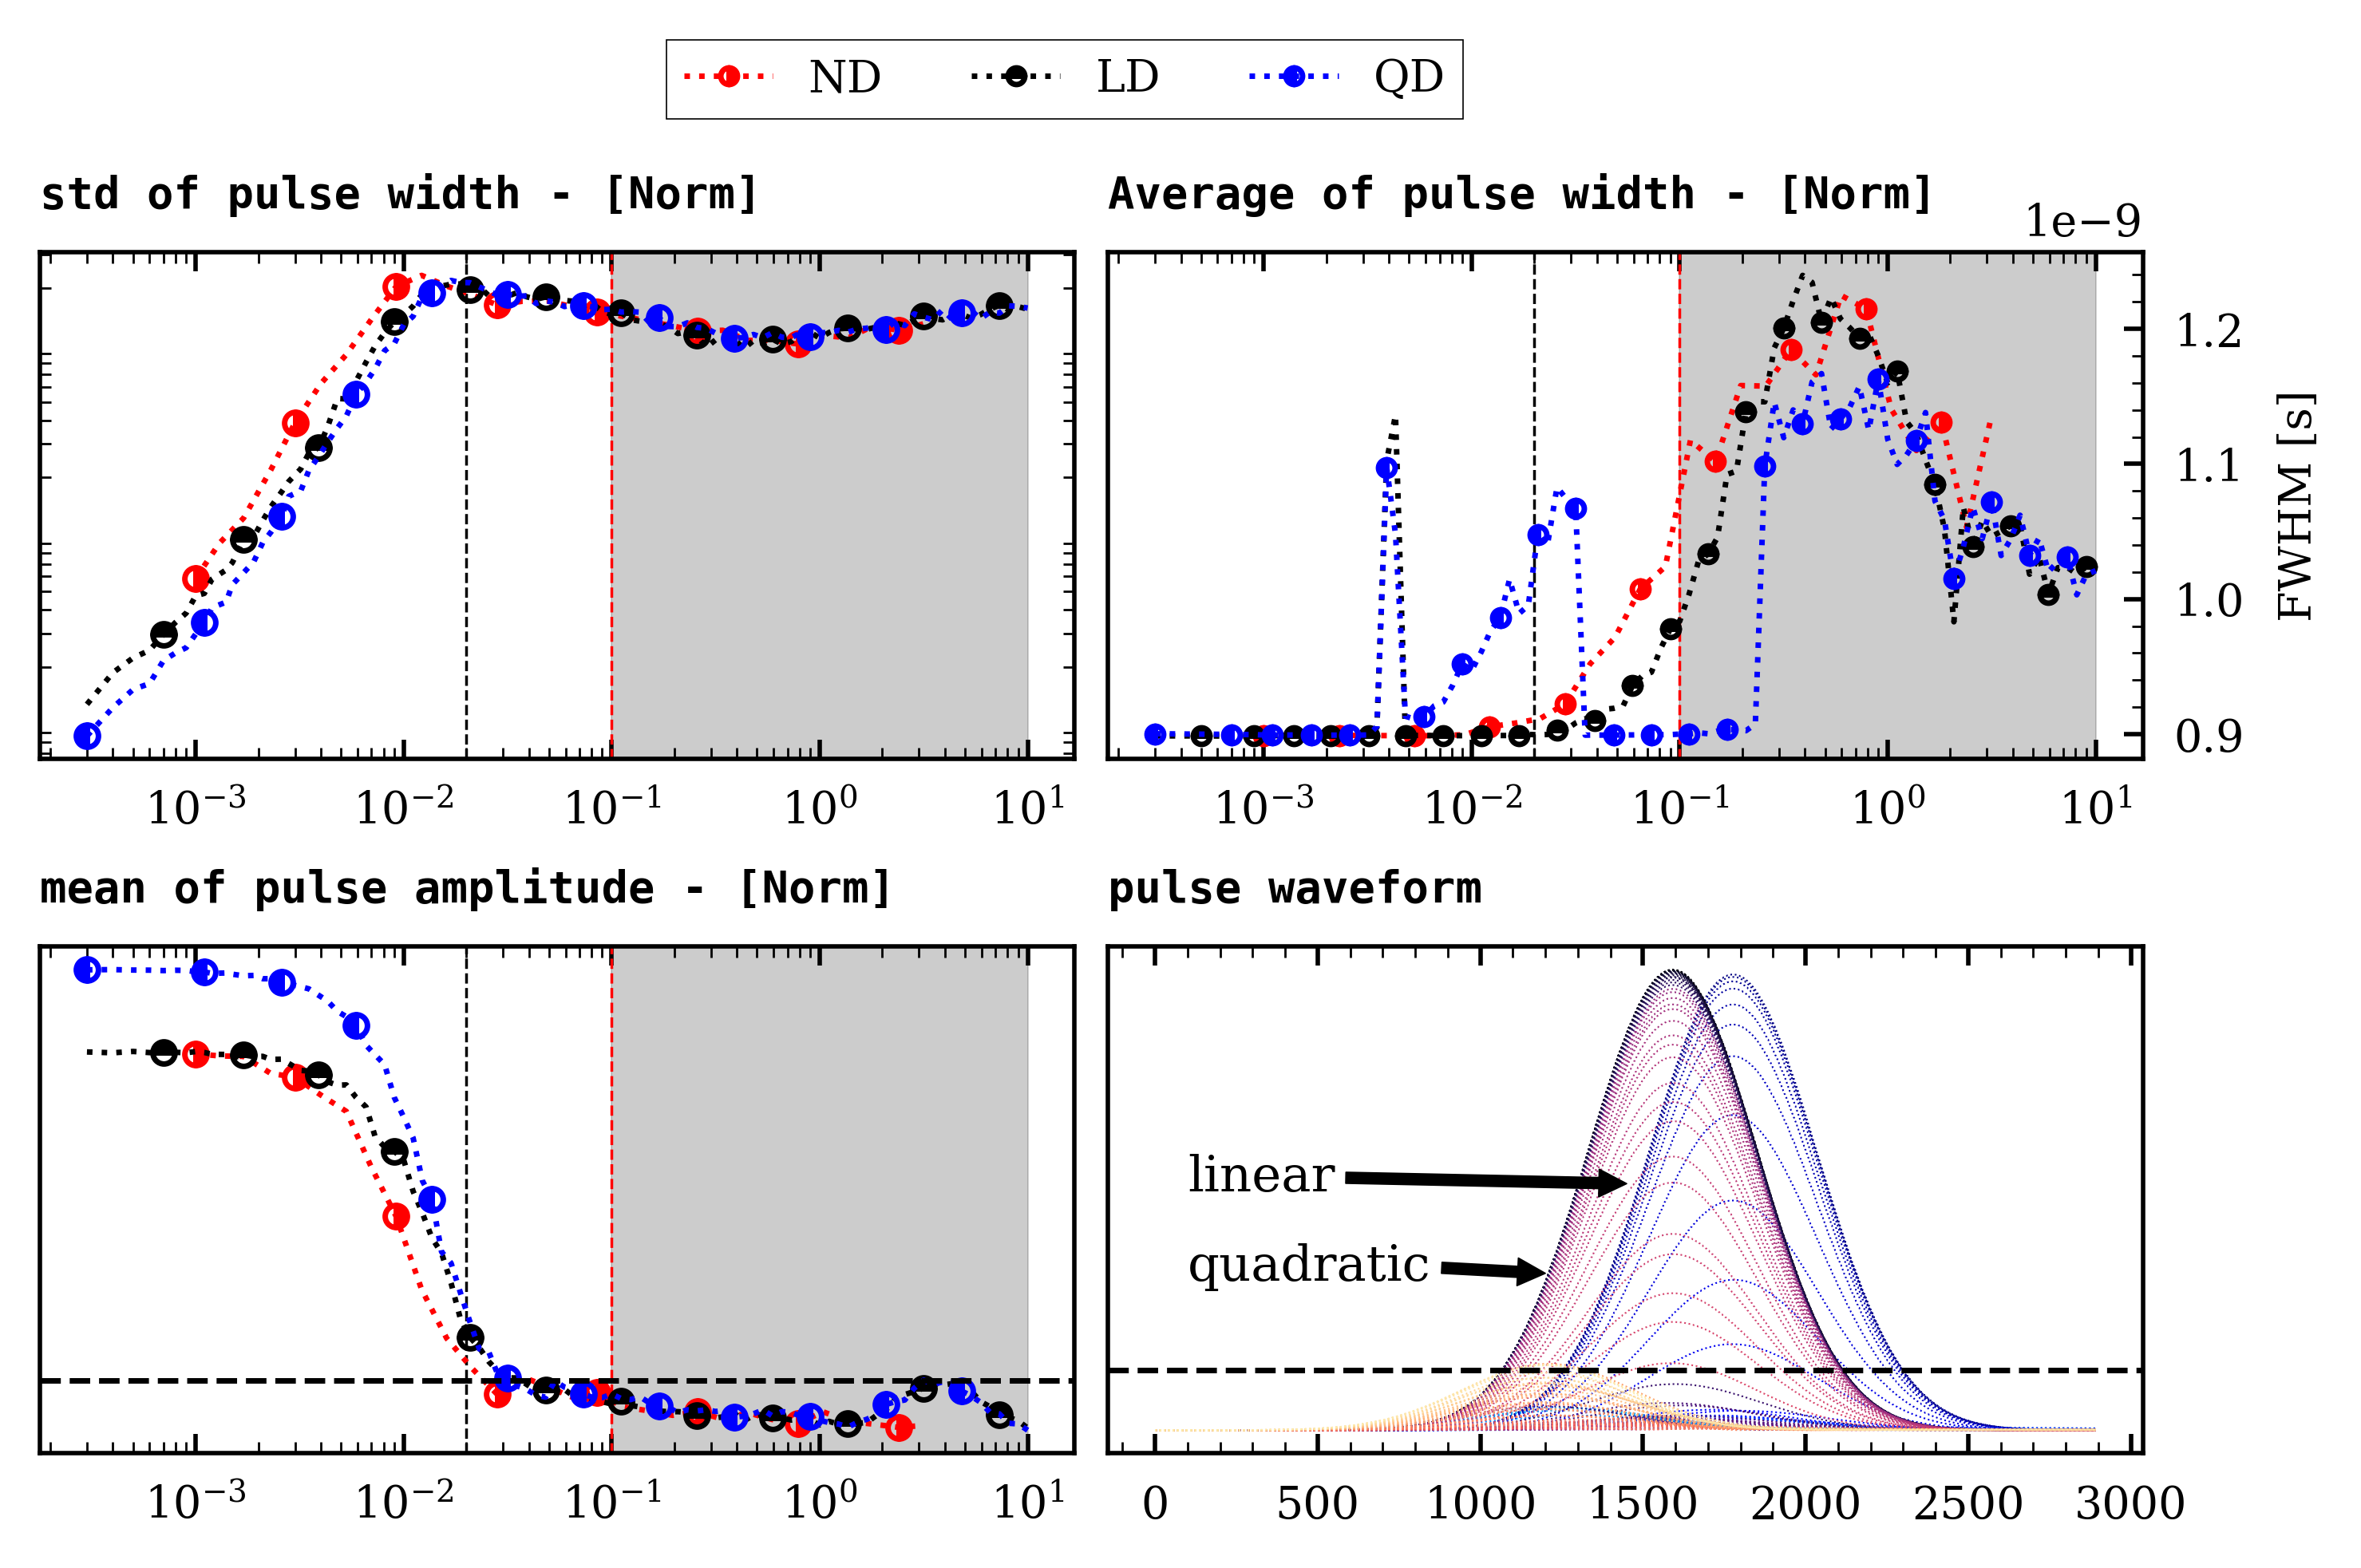
\includegraphics[width=1\linewidth]{./figures/pulse_params.png} %TODO : STD OF PULSE WIDTH WHY INCREASING
    \caption{Here we plot three differents metrics to characterize the pulse shape, the std of the pulse width, which is increasing (WHY), the average pulse width is increasing as intended due to the superposition of multiple scattered pulse, for the mean pulse amplitude, it's decreasing for the same causes, however let's note that after the transition regime the mean pulse amplitude seems to increase again reaching a maximum at the amplitude value $5$, the linearized turbulence turbulence density profile is also decayed from the simple linear background profile. This is easily understandable since we decrease the mean density turbulence amplitude in the plasma by linearizing the perturbation profile.
        One final thing to remark is the decay between the quadratic and the linear delays, indeed the quadratic profile has a little advance over the linear one. This is pssibly due to the concace shape of the background quadratic profile. Indeed, thanks to the concavity, it's much easier to turbulence to reach the cut-off layer, and to perturb it.}
    \label{}
\end{figure}

\begin{figure}[H]
    \centering
    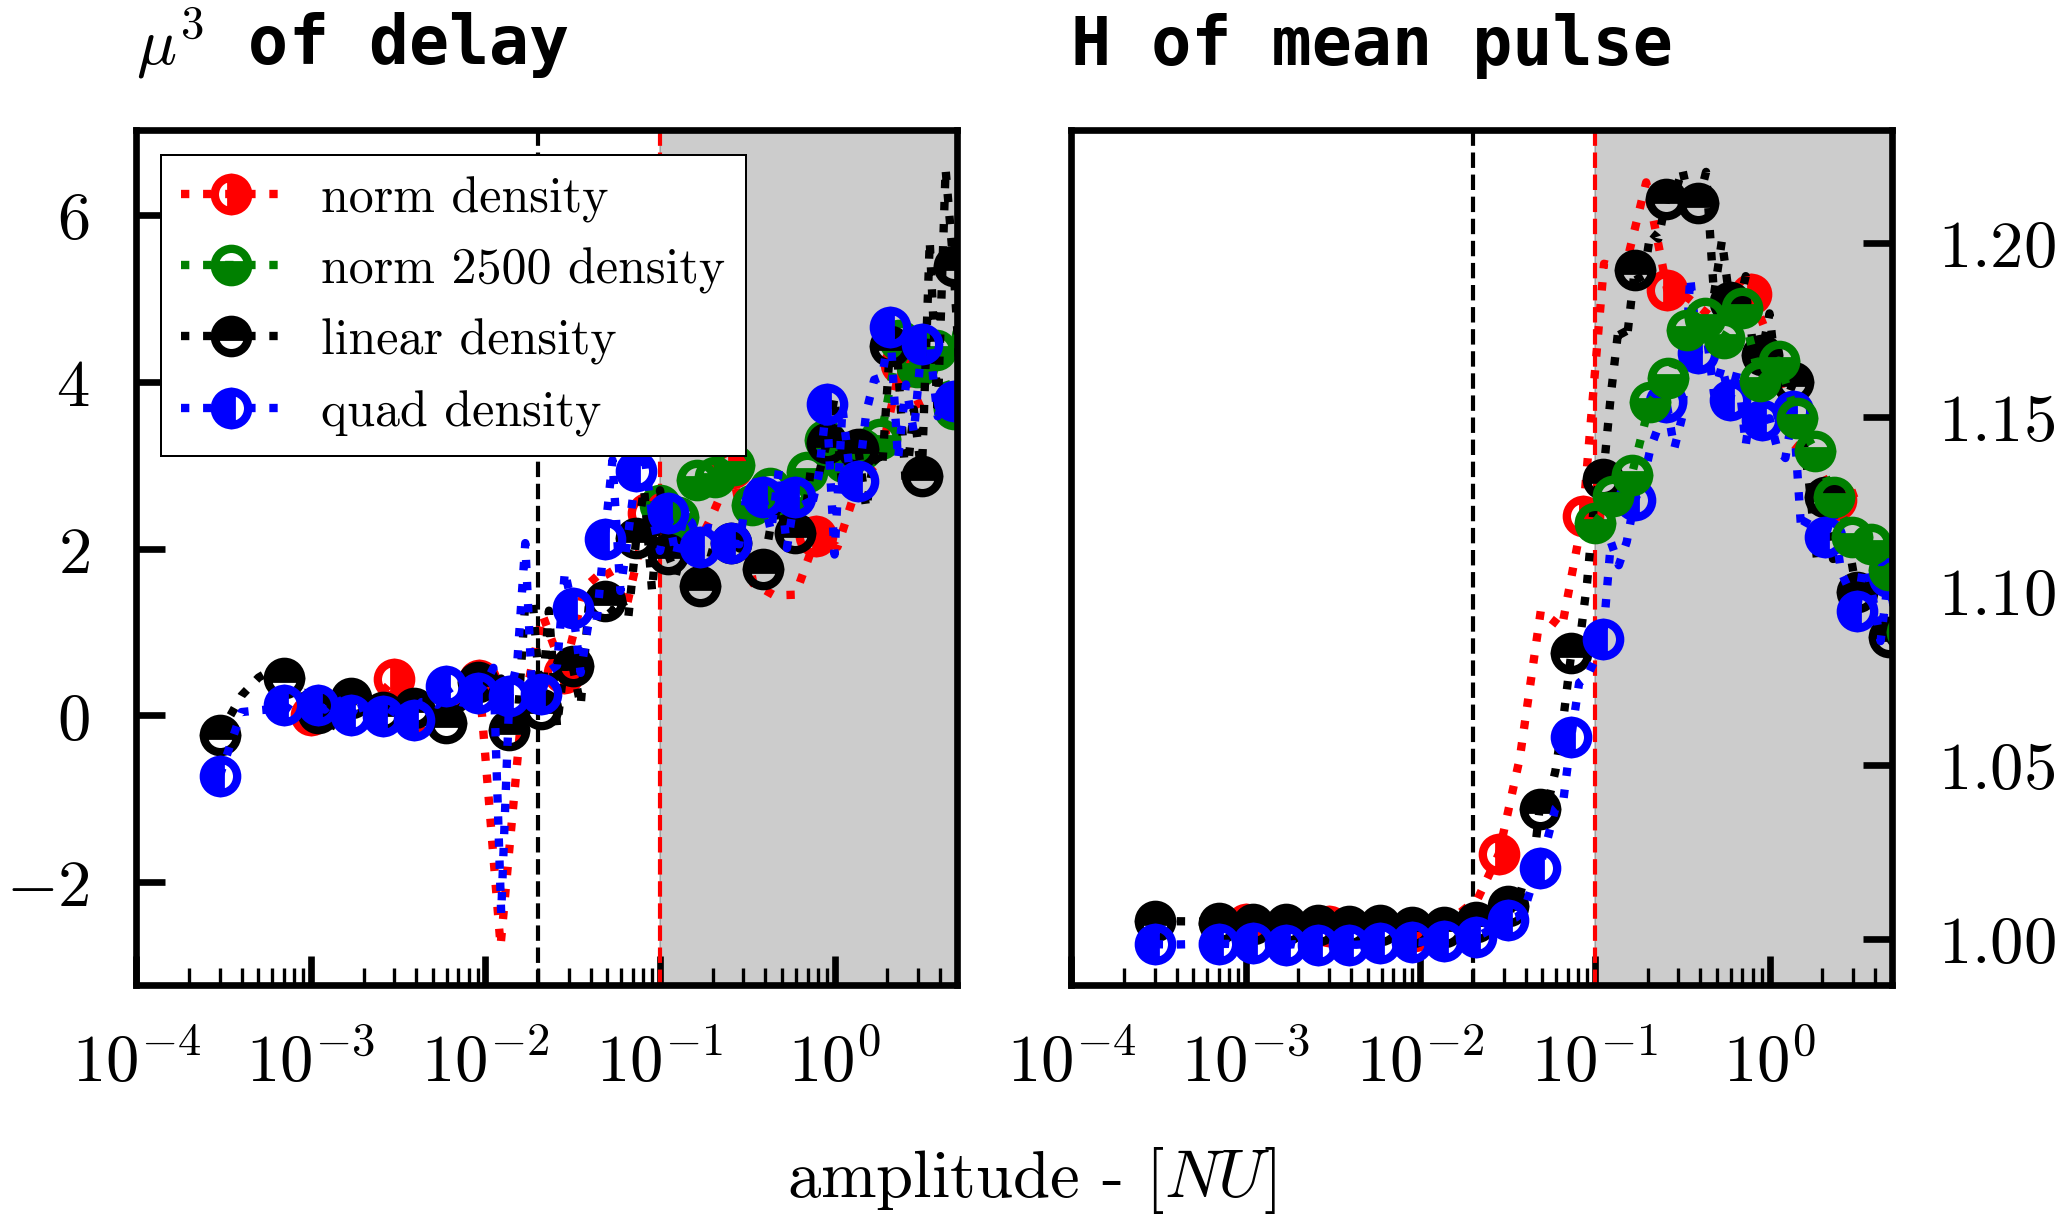
\includegraphics[width=1\linewidth]{./figures/skew_Hyst.png}
    \caption{skewness of the delay shape, for different background profile, and perturbation amplitude. The skewness is getting larger and larger for large perturbations, this is due to the presence of multiple scattering, and dispersive effects. The hysteresis of the pulse is calculating using the ratio of the right area over the left area of the pulse, this allows to see the asymmetry of the pulse shape which is a measurement of the skewness of the pulse.
        The true Skewness of the pulse does not unearth smoothly the transition regime, this is why it is not tackled here. }
    \label{}
\end{figure}

\begin{multicols}{2}
    \subsection{Gaussian fitting of the pulse}
    On way to see the deformation of the gaussian pulse is to track the relative error of the gaussian pulse with a gaussian fit. Furthemore, it allows to study the true gaussian standard deviation, mean and amplitude.
    This is shown in the following figure, where we plot the relative error of the gaussian fit, and the gaussian fit
\end{multicols}
\begin{figure}[H]
    \centering
    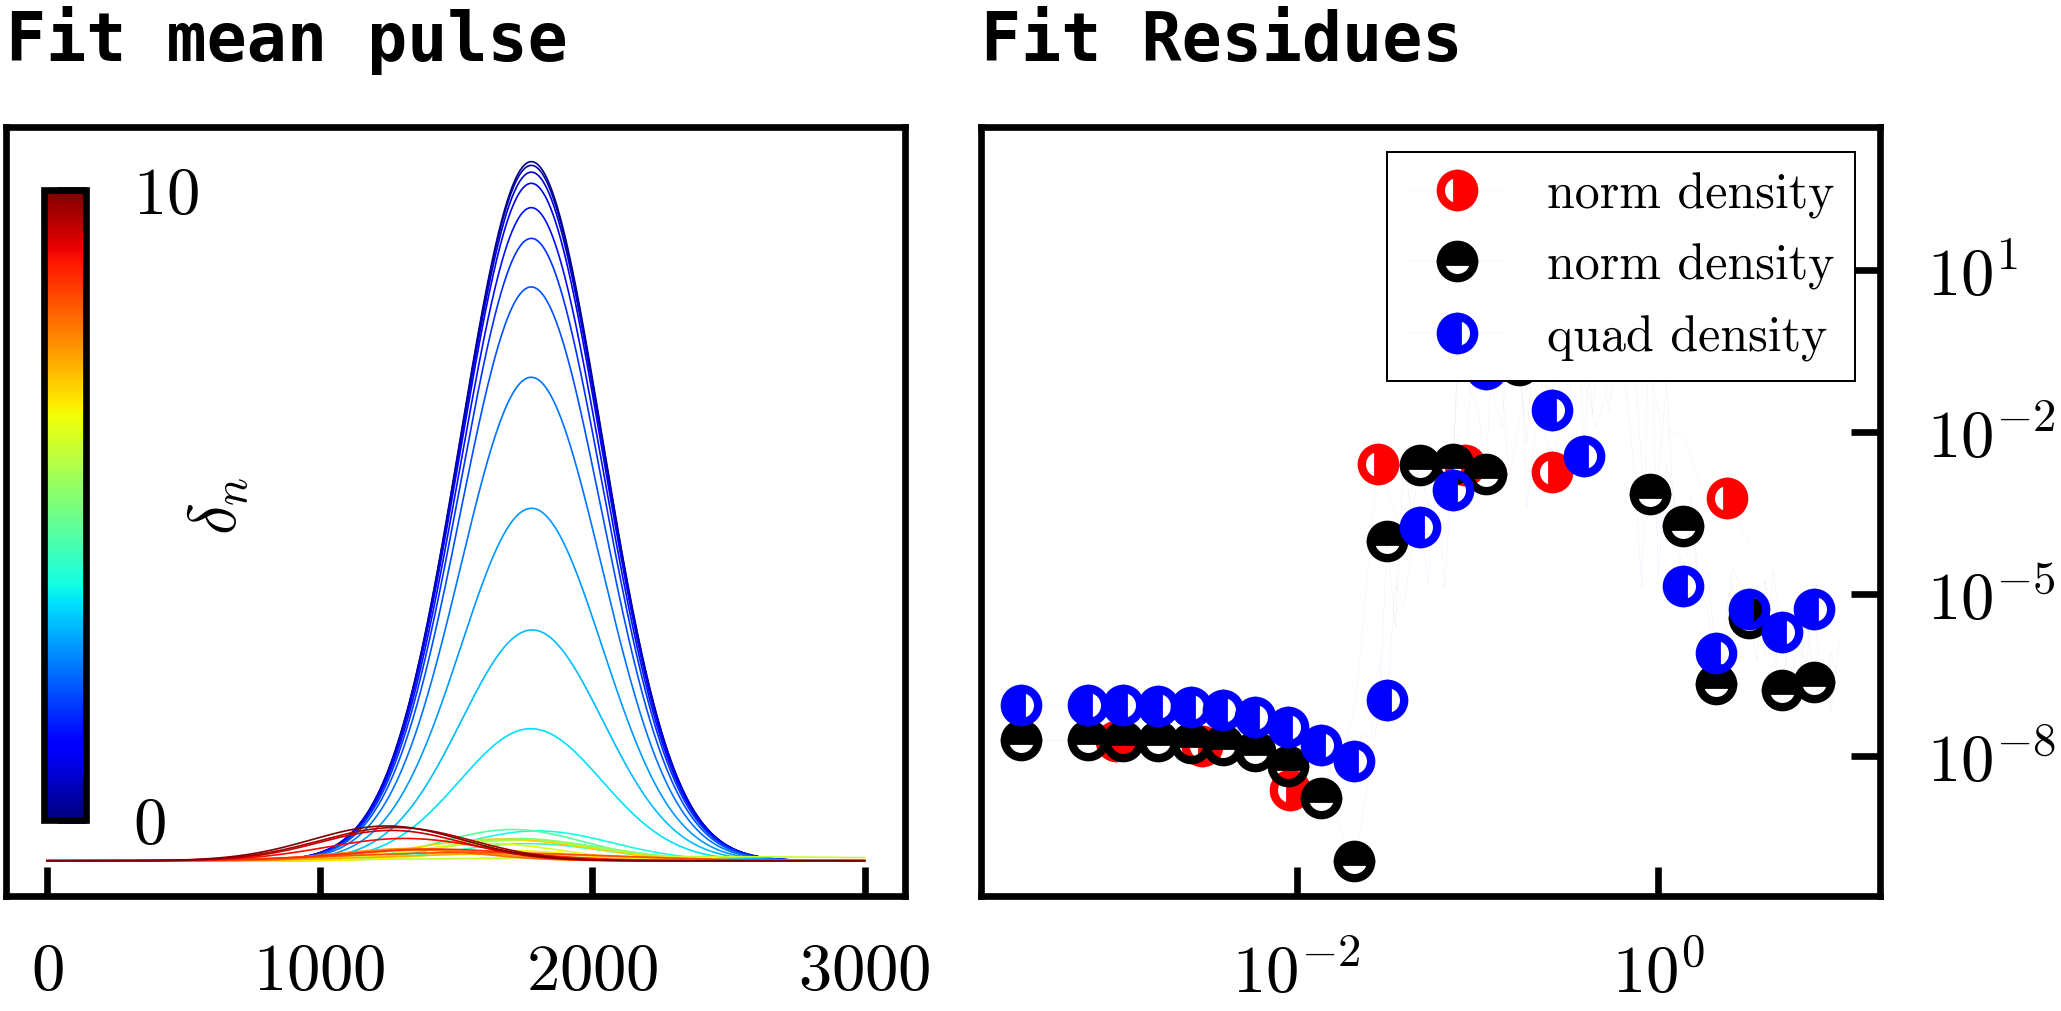
\includegraphics[width=1\linewidth]{./figures/gaussian_fit.png}
    \caption{The relative error of the Gaussian fit (residuals ponderated by the size of the respective pulse amplitude) is getting large for the transition zone of the pulse shape, and seems to decline for very large turbulence. However we have to find smooth metrics to characterize the transition, and not a pseudo-random one to have better predictions in the next part.
        The gaussian parameters are also good quandidates and are plotted in the next figure }
    \label{}
\end{figure}

\begin{figure}[H]
    \centering
    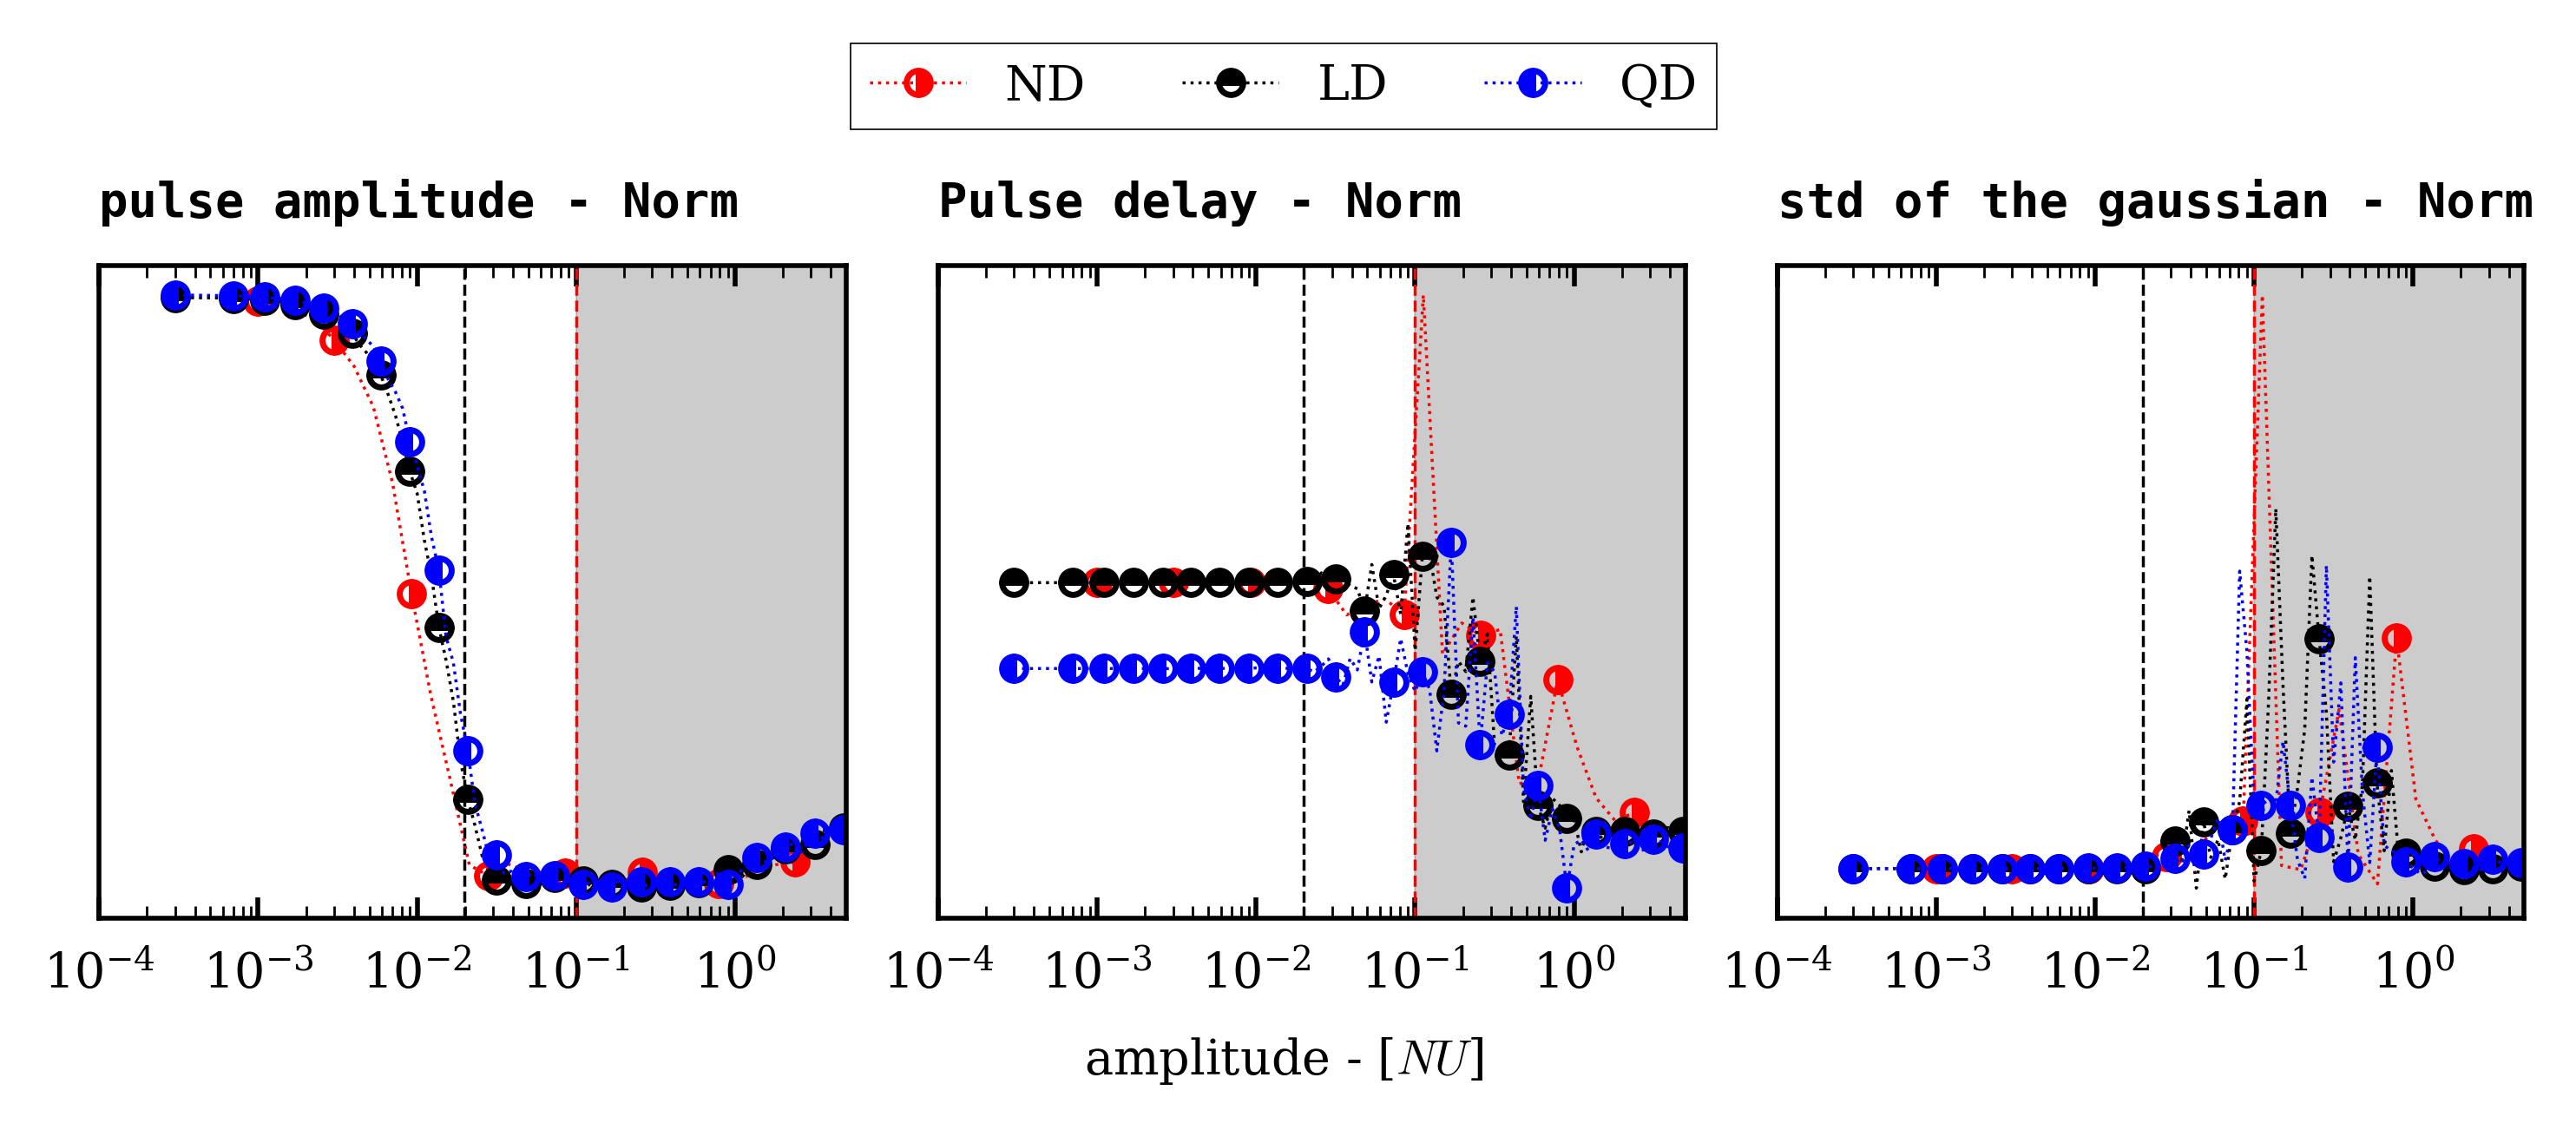
\includegraphics[width=1\linewidth]{./figures/gaussian_Params.png}
    \caption{Gaussian pulse delay and standard deviation have chaotic behavior during the transition regime, this made them not relevant candidate for the next study. However lets note that the gaussian pulse ampliutde,
        have quite a smooth behavior, but unearth a plateau during the non linear linear transition, which might not ne a good option, even if at large amplitude we capture the same behavior as for the non gaussian amplitude.
        In a much cleaner way, indeed it's clearly increasing, this might be interesting to study the highly non linear regime.}
    \label{}
\end{figure}

\begin{multicols}{2}

    \section{Model collapses}

    As shown previously, the 1D model collapses for large perturbations. The goal of this chapter is to facilitate the deduction of the perturbations properties just from the typical study of the delayed pulse.
    Our goal will be to predict the perturbation amplitude, their typical correlation length and the original delay of the probing wave $\tau_0$ without any perturbation. Using previous results, it might be quite simple to isolate the original delay and the turbulence amplitude, but the correlation length is a more difficult parameter to isolate, and seems to play a great role in the pulse properties.

    \chapter{Non linear regime study}
    The non linear regime is a much more difficult regime to study, indeed the perturbations are large enough such that the cut-off layer is strongly perturbed, and the WKB approximation cannot be applied. The main goal of this approach is to find a way to link the plasma density perturbations to the reflected pulse delay. To retrieve some information about the pulse delay we will use a statistical approach to get rid of the randomness implies by the perturbations considerations.

    \section{1 dimensional study}
    To test the validity of the machine learning approach, let's try to tackle the non-linear regime using the 1D dimensional approach. The 1D study didn't give the ability to retrieve information in this regime.
    To do so we will use the same approach as for the linear regime, but with a much larger perturbation amplitude. Different profiles will be used to see if the model succeeds in predicting the wanted features.

    \subsection{Density profiles}
    Through this study multiple density profiles have been used, to see if the model can generalize the results, and to see if the background profile has a strong influence on the model results. Multiple combinations of background and turbulence profile have been used through linear to quadratic background profile with linearly normalized or exponential normalized perturbation profile.
    The most complex case studied was the quadratic background profile combined with am exponential linearized turbulence profile.
    The normalization follows : $$\delta n = a\tilde{\delta n}\frac{n(x)}{n_c} \exp(\frac{L-x}{L}) $$

    % \begin{tikzpicture}
    %     \begin{axis}[
    %             legend pos=north east,
    %             title=Turbulence profile,
    %             axis lines = box,
    %             xlabel = $\frac{x}{L}$,
    %             ylabel = $\frac{\delta n}{n(x)}$,
    %             variable = t,
    %             trig format plots = rad,
    %             ymin=-4,
    %             ymax=4,
    %         ]
    %         \addplot [
    %             dashdotdotted,
    %             domain=0:1,
    %             samples=70,
    %             color=black,
    %         ]
    %         {exp( (1 - x) / 1)};
    %         \addlegendentry{$n_{c1}$}
    %         \addplot [
    %             dashdotdotted,
    %             domain=0:1,
    %             samples=70,
    %             color=black,
    %         ]
    %         {-exp( (1 - x) / 1)};
    %         \addplot [
    %             dashed,
    %             domain=0:1,
    %             samples=70,
    %             color=black,
    %         ]
    %         {1/x};
    %         \addlegendentry{$n_{c2}$}

    %         \addplot [
    %             dashed,
    %             domain=0:1,
    %             samples=70,
    %             color=black,
    %         ]
    %         {-1/x};

    %         \addplot [
    %             domain=0:1,
    %             samples=70,
    %             color=black,
    %         ]
    %         {1};
    %         \addlegendentry{$n_{c3}$}
    %         \addplot [
    %             domain=0:1,
    %             samples=70,
    %             color=black,
    %         ]
    %         {-1};

    %         \addplot[
    %             domain=0:1,
    %             samples=70,
    %             color=red,
    %         ]
    %         {0.3*gauss(0,0.1) + 0.2*gauss(0.7,0.08) + 0.2*gauss(0.5,0.1) + 0.25*gauss(0.9,0.05) + 0.1*gauss(0.2,0.3) + 0.15*gauss(0.4,0.1)- 1};

    %     \end{axis}
    % \end{tikzpicture}
    This exploration of the density profile is motivated by the fact that at the edge of the plasma, the relative amplitude of the turbulence profile is higher than in the core of the plasma.
    The simple linearization of the turbulence profile gives a constant envelope, wheras the non normalized one gives a divergent one at the edge. One solution was to introduce an exponential factor to the normalization.

    \subsection{Datasets building}
    \begin{center}
        \begin{tabular}{ccccc}
            \toprule
            \multicolumn{5}{c}{Parameters range}                     \\
            \cmidrule{1 -5}
            $\delta n$     & $l_{cx}$-[cm] & L-[cm]   & $N_x$ & n    \\
            \midrule
            $[1e^{-3}, 1]$ & $[0.1,1]$     & $[7,20]$ & 5000  & 1000 \\
            \bottomrule
        \end{tabular}
    \end{center}

    \begin{figure}[H]
        \centering
        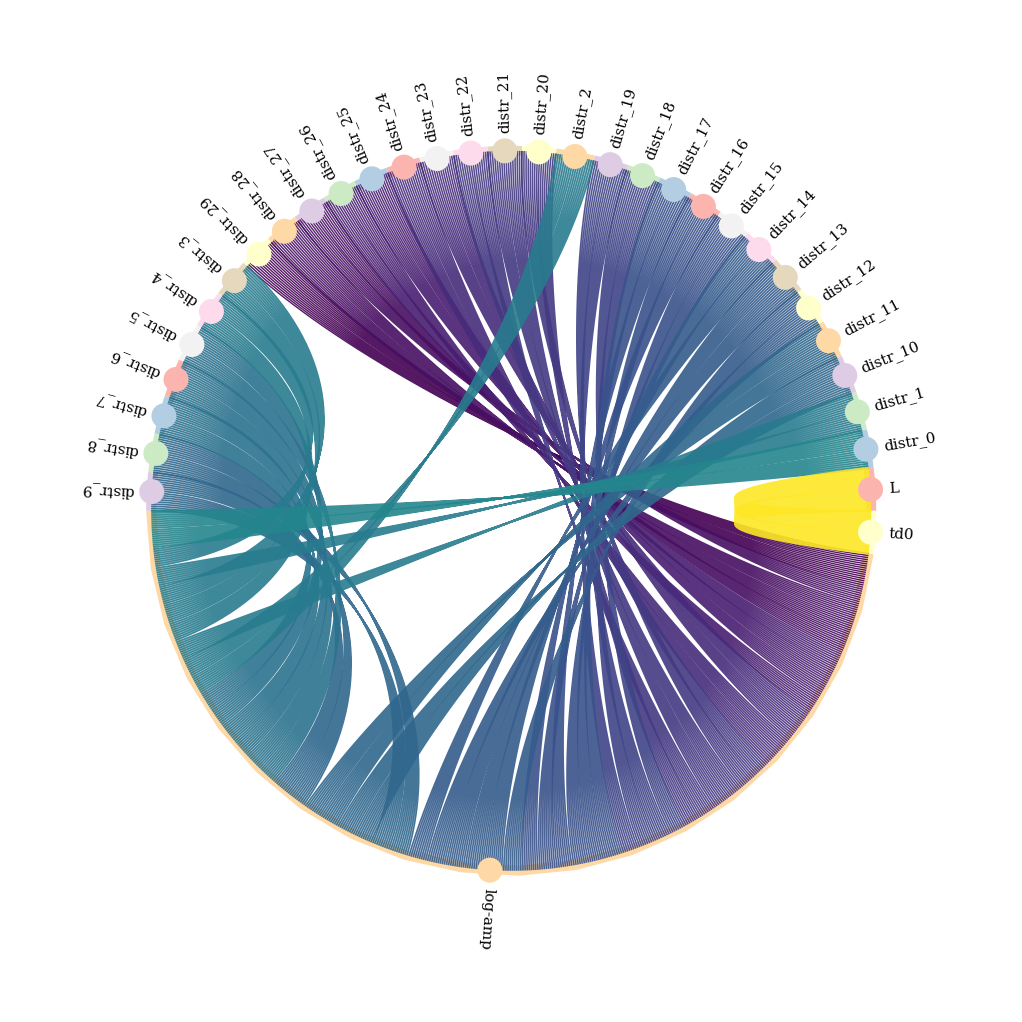
\includegraphics[width=1\linewidth]{./figures/chord.png}
        \caption{Chord plot of Correlation between Variables, every correlation between quantiles are omitted. The strong correlation between $L$ and $\tau_0$ is correct in our dataset, but we want our model to get rids of this relation to avoid getting wrong results when L will stand for the gradient scale at the cut-off layer.
            Our model should be able to get $\tau_0$ with only the statistical properties of the delay.}
        \label{}
    \end{figure}


    For each density profile we compute the integrated delay of many samples to have a statistical overview of this latter. One way to tackle the problem was to study the binned delay but is leads to a strong collapse when we removed the perefect linear dependency between $td_0$ and $L$. An easier method was to study the quantiles of the $td$ distribution, and it leads to qualitiative results, without the collapsing of the prediction when introducing a little random shift in the delay distribution.
    We were using a 30 quantiles discretization of the delay distribution which leads to a 32 dimensions input dataset, and a 2 dimensions output dataset, the perturbation amplitude and the original delay of the probing wave $\tau_0$. Then all datasets corresponding with each density profiles were assembled and normalized using a Z-score normalization, to have a much global undterstanding of the model.
    Let's recall that the goal of this approach is to predict the perturbation amplitude and the original delay of the probing wave $\tau_0$, using the statistical property of the delay, and the correlation length in the $x$ direction, in this 1d model.


    \subsection{Regression model}
    To tackle this problem, we tested several regression models, from GradientBoosting Mutlioutput model to random forest.
    The best results were obtained using a RegressorChain GradientBoosting model with a final score on the test set of 0.99, however we succeed in getting a beter score, obtaining a near perfect model, using a tricky RegressorChain StackedRegressor model packing four different regressor model,
    \textbf{GradientBoosting, RandomForest, KNeighbors, GaussianProcess}, this model is then trained to predict the perturbation amplitude and the original delay of the probing wave $\tau_0$, using the four models results, it is a much more complex and versatile model, with an absolute error of 0.99 out of the test set.
    To have beter vizualization of the model results, we can plot the predicted log-amp of the test set over the true log-amp. The dispersion of point around the identity will then give us an overview of the model quality.

    To test if the same model can learn to retrieve the $\tau_0$ value only from the delay distribution, we trained another model using the same dataset omitting L, the results are clearly collapsing with a $R^2$ score of 0.6 without or with a random shift in the delay distribution, we also showed that putting the amplitude in the input datasets leads to significantly better results with a $R^2$ score of 0.82, this is tackled in the 2d output model without the \textbf{RegressorChain}[cite]. This was intended since the turbulences are responsible in a shift of the cut-off.

    \subsection{Results}
    The models are tested for every case on the test dataset, and on the 2d output simulations to see if our 1D training model can be generalized to 2D data.
\end{multicols}
\begin{figure}[H]
    \centering
    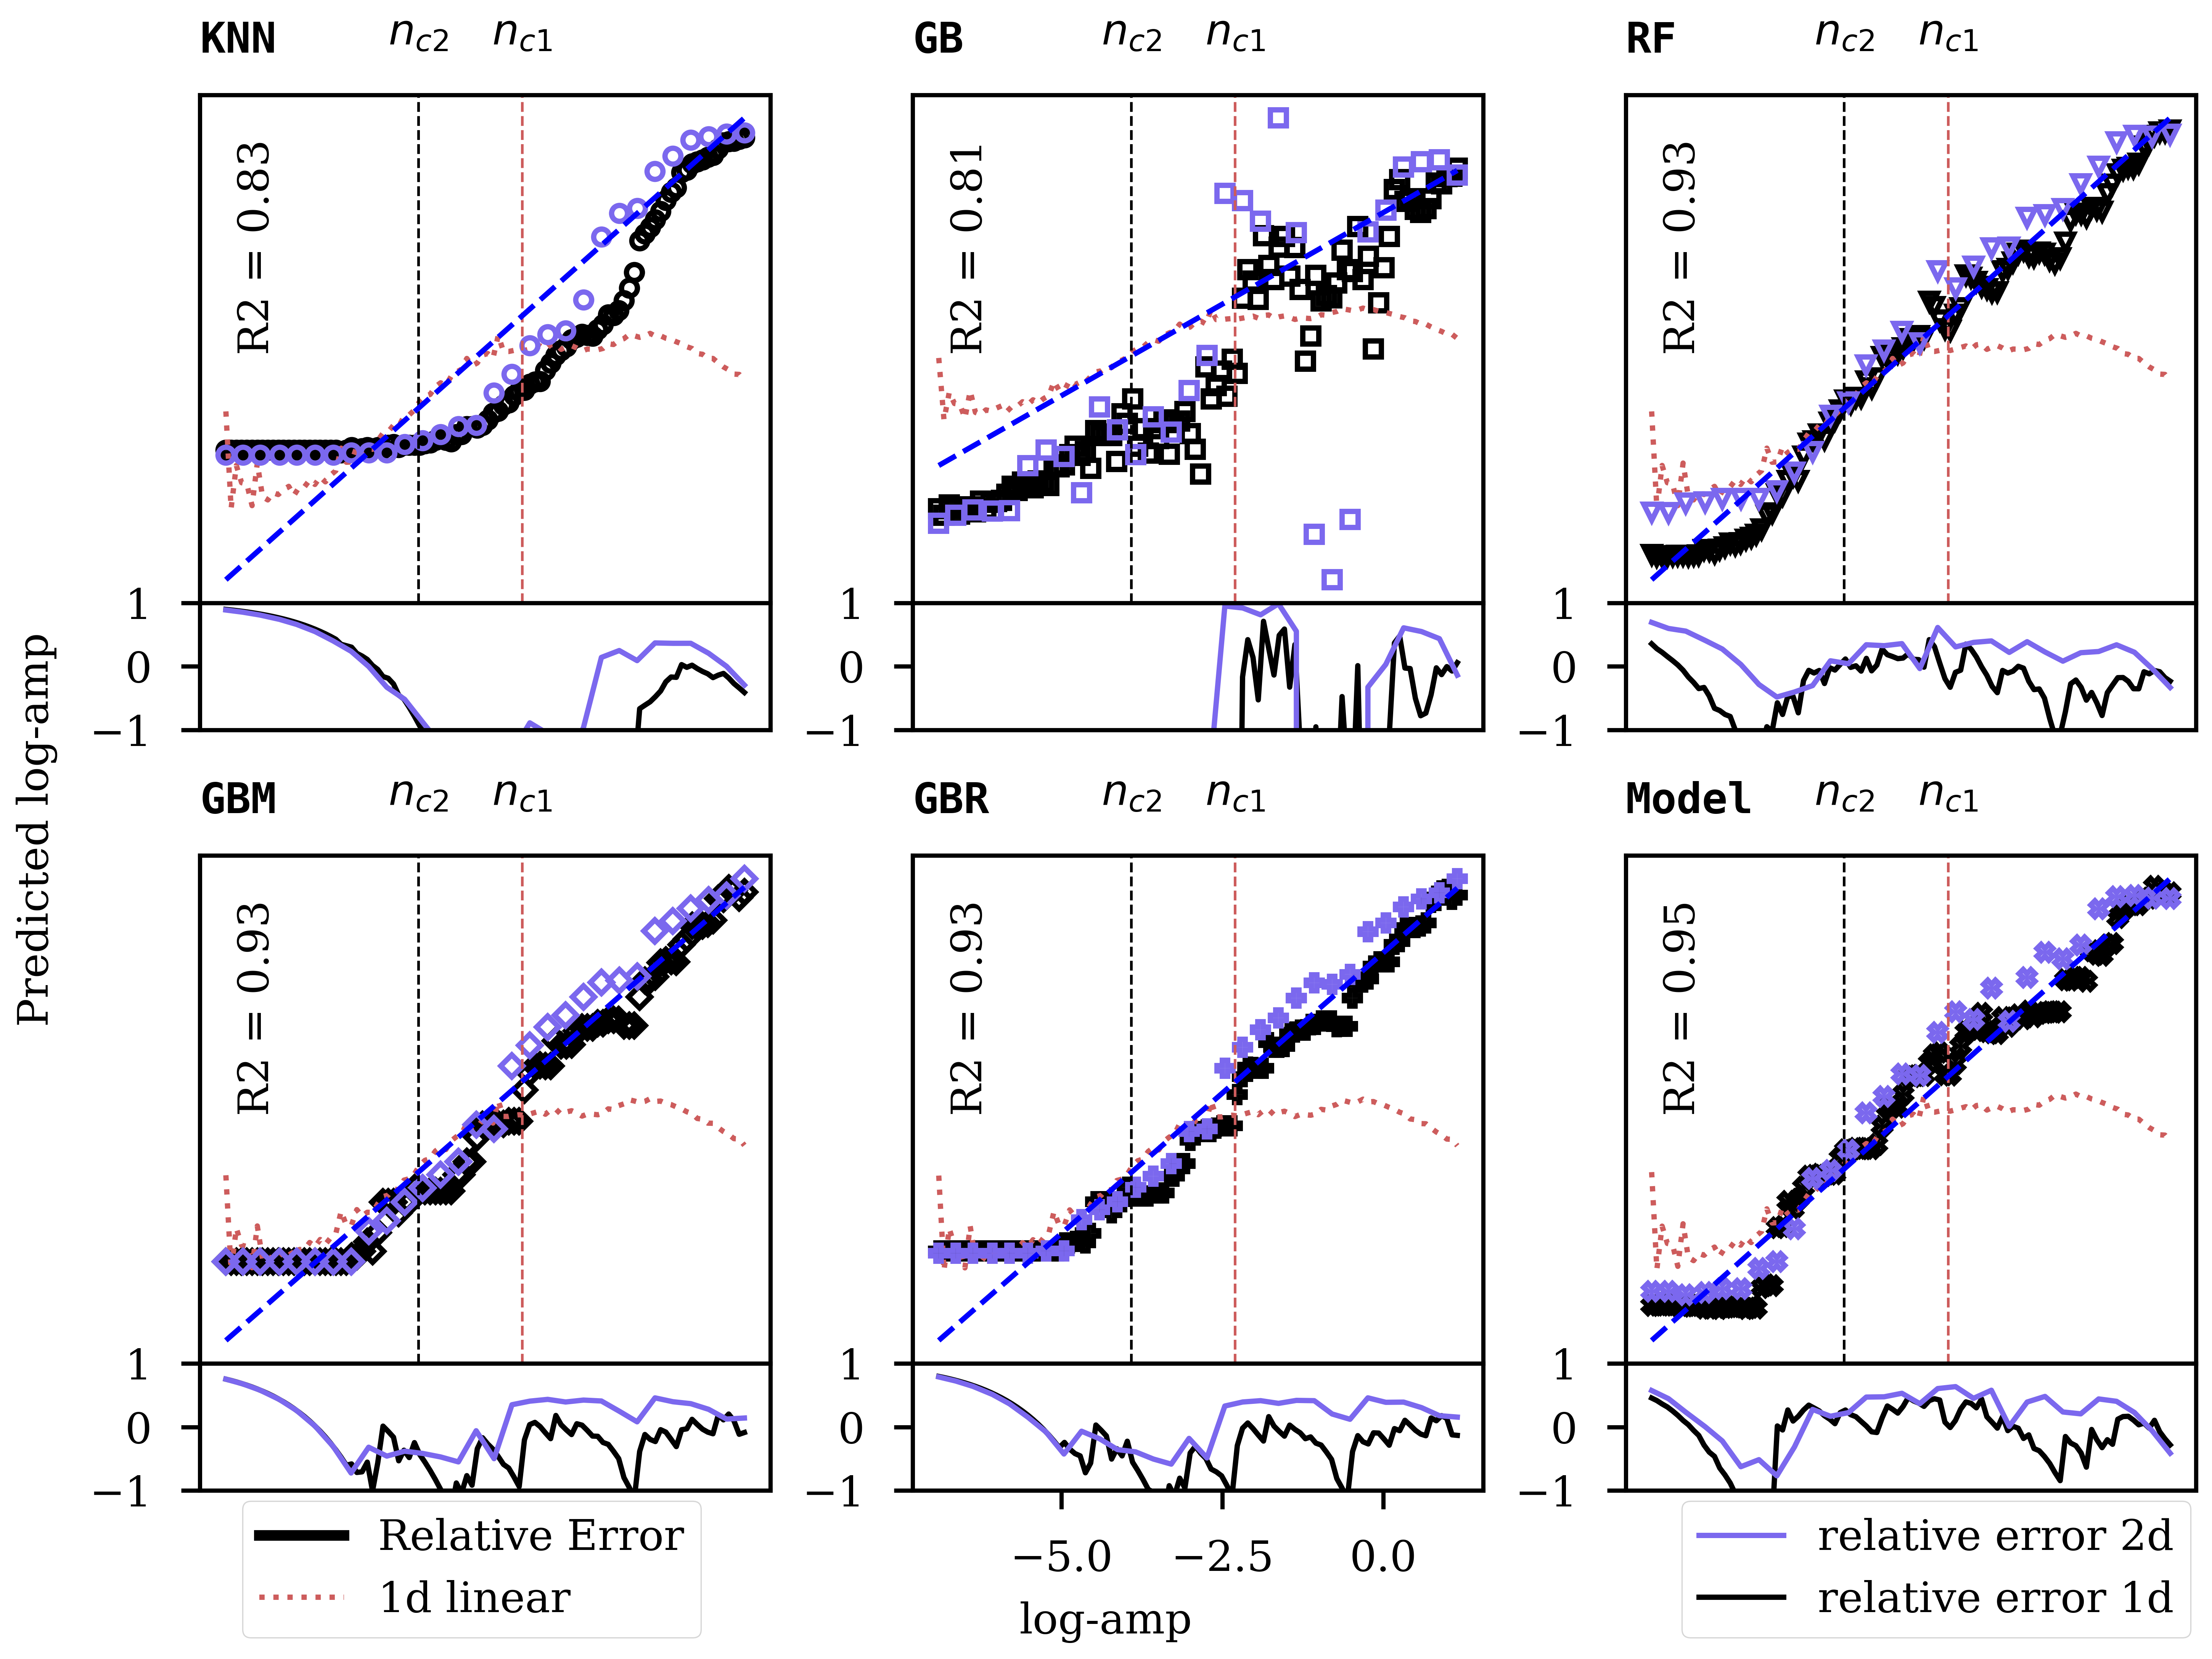
\includegraphics[width=1\linewidth]{./figures/amp_amp_final.png}
\end{figure}
\captionof{figure}{The predicted amplitude versus true amplitude unearths several interestings points. First our stacked regressor model is able to predict the amplitude with a very high accuracy (black plot), and the predicted delay versus the true delay is quite good for all ranges of amplitude, even for extreme-amplitude perturbations, whereas or previous analytical model is far from being able to even predict the oreder of magnitude of the amplitude at high amplitude (for $\delta n > n_{c1}$).
    Surprisingly the model is able to generalize is learning to the 2d Simulation extremely well (blue plot), with a relative error on the amplitude of less than 10\% for interesting amplitudes}


\begin{multicols}{2}
    One other way to see physically the good quality of the model learning is to plot the mean value of $\tau$ over the value of the log-amp.
    Indeed in the 1D analytics approach we supposed that $\tau_0 = < \tau >$, this hypothetsis is broken for high amplitudes, so the theoritical value should depend on the amplitude, whereas $\tau_0$ does not depend on amp, since is the value of the delay without amplitudes.

\end{multicols}
\begin{figure}[H]
    \centering
    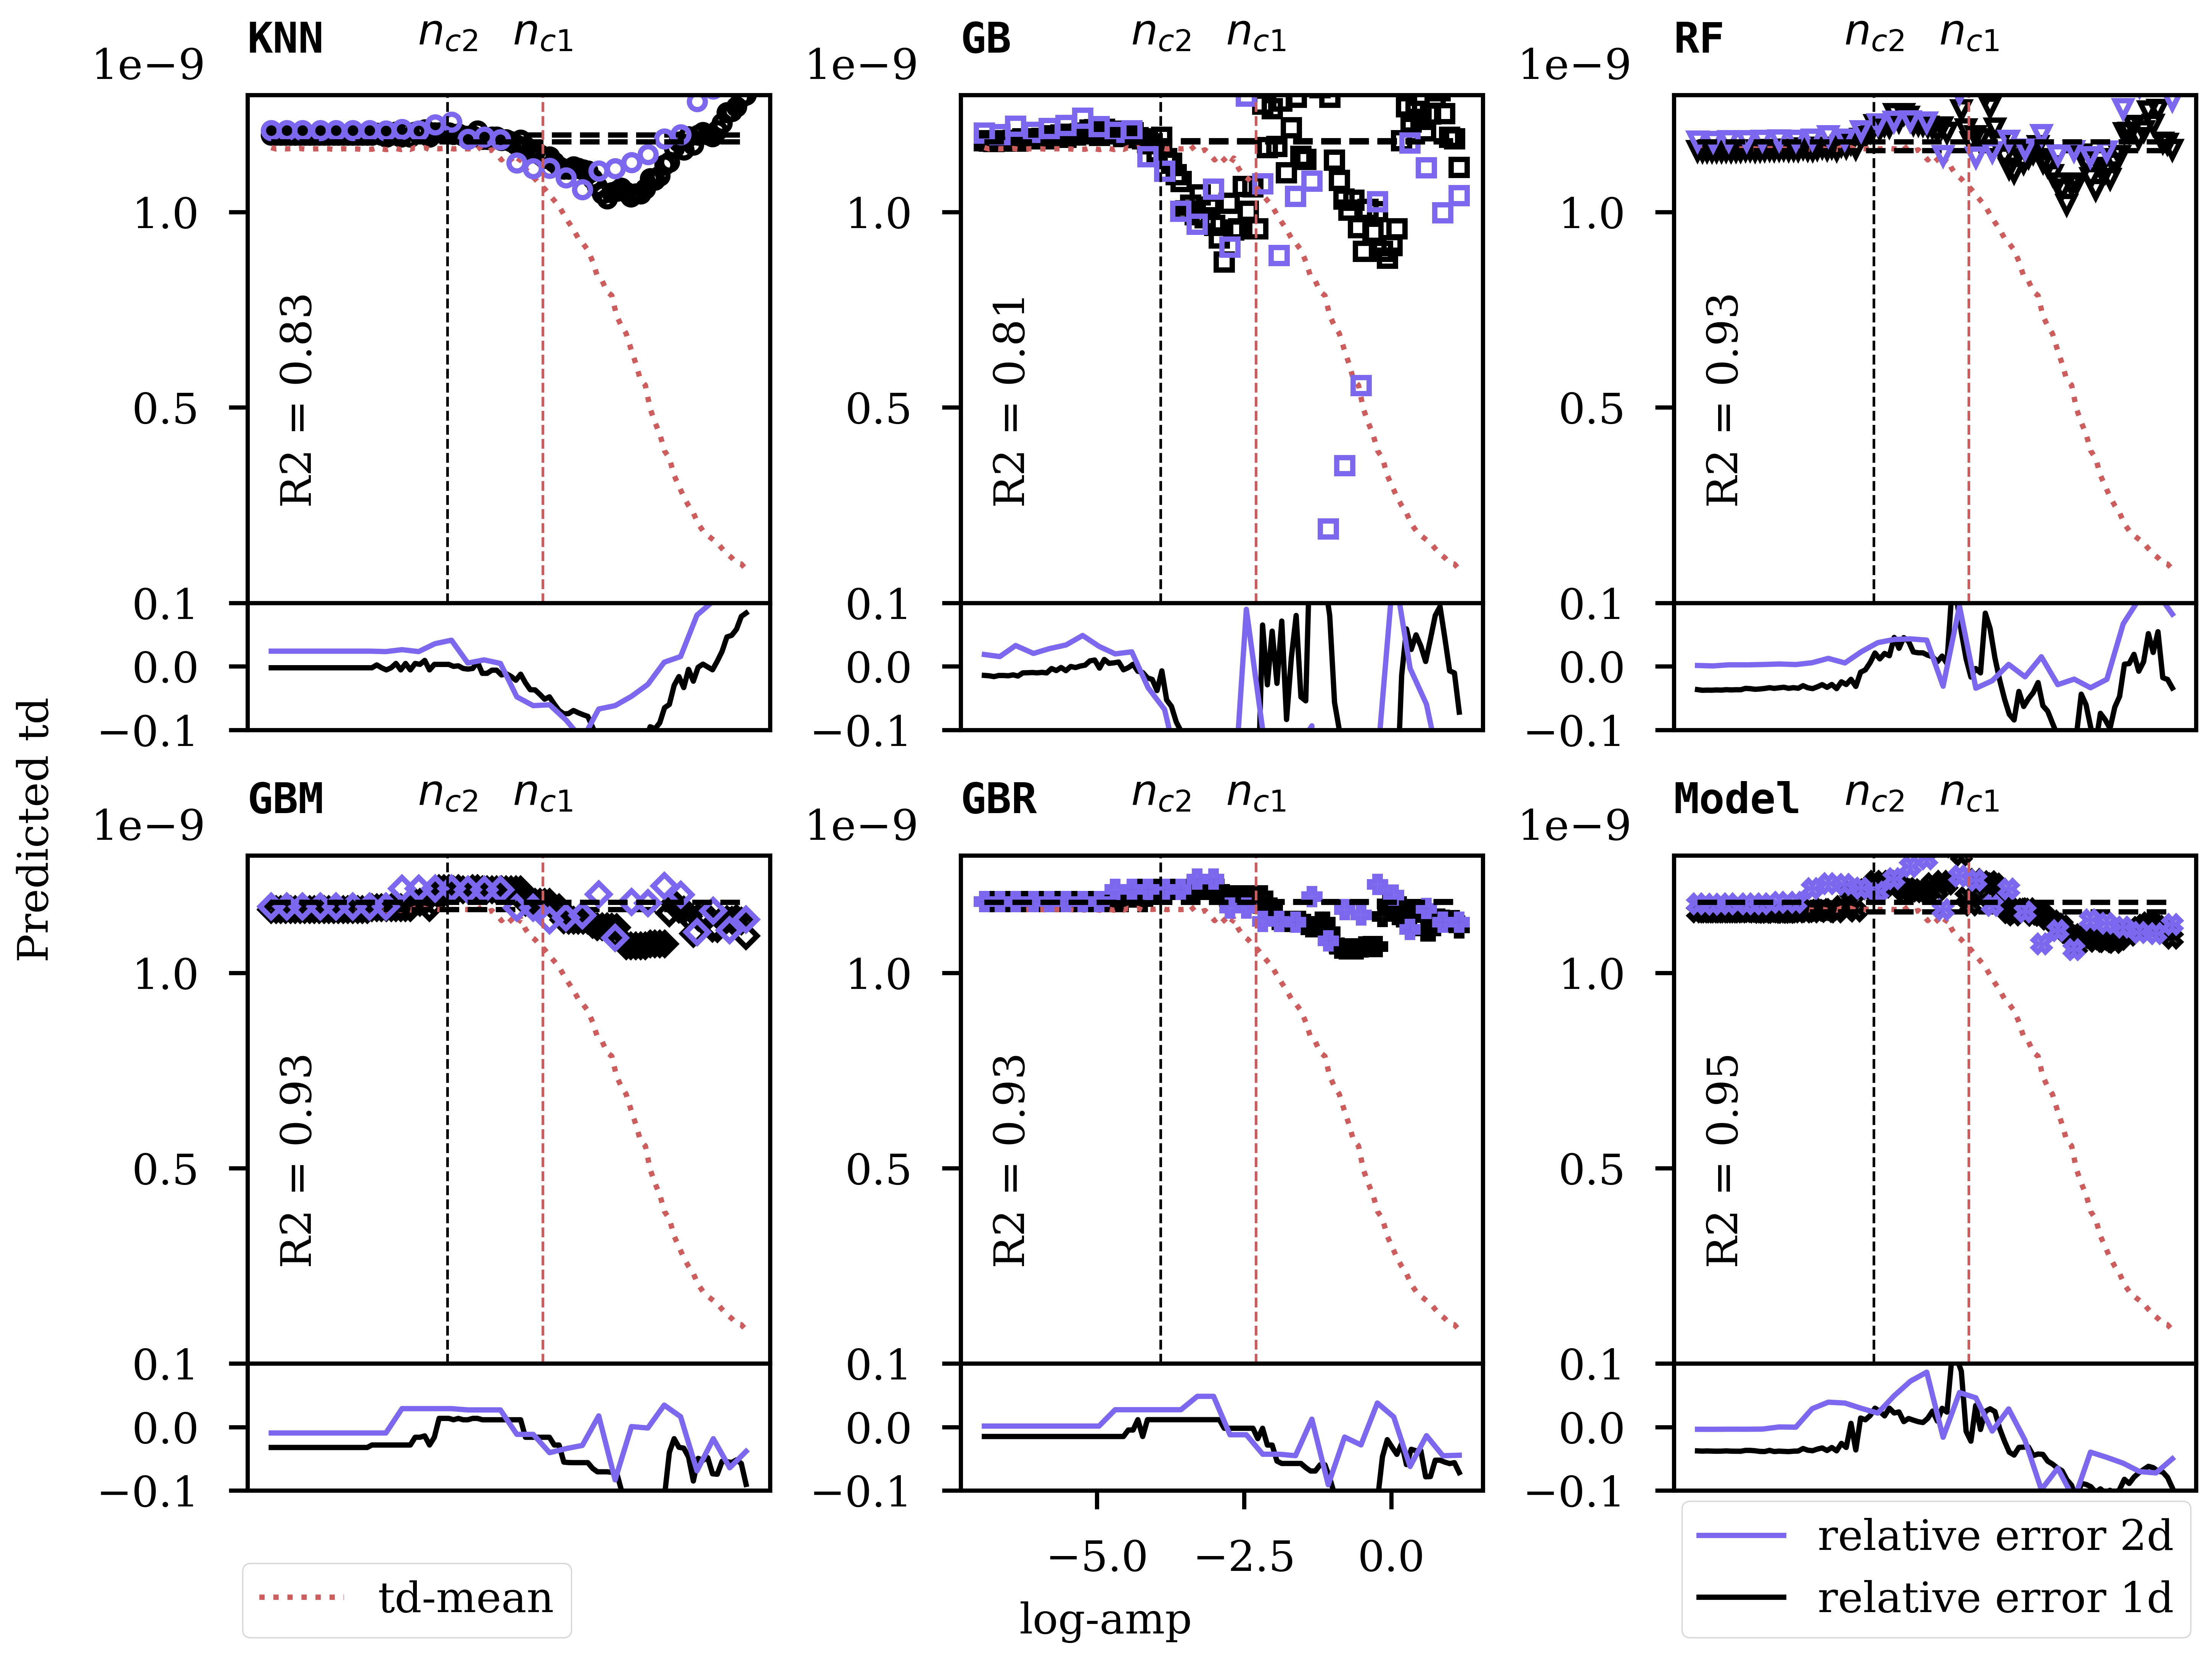
\includegraphics[width=1\linewidth]{./figures/delay_amp_final.png}
    \caption{.}
    \label{}
\end{figure}

\begin{multicols*}{2}
    Test on combined datasets

    Test on shifted td0 and td bins to avoiding the model to learn just with L dependancy of td0.
    but on the relations between td bins and td0

    Test on quantile data whether than binned data, to avoid the scale learning by the model

    TD0 with shift train model, test with 0 shift model

    1D training applied to the 2D simulations, shifted to the mean of the 1D model, quite good results

    2D training on new simulations

    2D training on curved profile (or flat curved profile)

    2D training on small angle incidence probing beam
\end{multicols*}
\begin{multicols*}{2}


    \section{2 dimensional study}
    \subsection{Datasets building}
    \begin{center}
        \begin{tabular}{cccc}
            \toprule
            \multicolumn{4}{c}{Parameters range}                            \\
            \cmidrule{1 -4}
            $\delta n$     & $l_{cx}$-[cm] & $l_{cy}$-[cm]   & $ro$-[cm]    \\
            \midrule
            $[1e^{-3}, 1]$ & $\{1, 0.5 \}$ & $\{0.5,2,30 \}$ & $\{1,4,10\}$ \\
            \bottomrule
        \end{tabular}
    \end{center}
    To deal with these multiple parameters, we will use a machine learning approach, trained on a datasets of simulated pulse shape, and delay for multiple ranges of value of $\delta n$, $l_{cx}$, $l_{cy}$ and beam size $ro$.
    To build this datasets we will based our apporach on the previous results, where we extracted the best hyperparameters candidate for both computations speed and accuracy. The datasets will be built using the linear normalized perturbation profile, and a number of sample $N_s = 500$, the $\tau_0$ will be compute for each combination of parameters, even if it should not depend on correlation lengths and amplitudes.

    - REDUCTION OF BM AND LCX CORR MATRIX
    - PLOT WITH ALL THE CORR MATRIX
    - USE SPIKEWIZARD
    - LCy PARAMS FOR 2D with 1D COMPARISON
    - 2D MODEL TRAINING
    - 2D MODEL TESTING (AMP AND TD0)
    - 2. Histogram of residual
    - LEVERAGES
    \subsection{Gaussian spectrum of the turbulences}
    The gaussian spectrum is the most simple way to model the turbulence, and was used as first approximation to see if the model could integrate the dependancy of the diffrent correlation length.
    The gaussian distribution of the wave vector is given by the following :

    \begin{figure}[H]
        \centering
        \includegraphics[width=0.7\linewidth]{example-image}
        \caption{Gaussian Power Spetrum and correlation length measurements}
        \label{}
    \end{figure}

    \subsection{Power Spectrum of the turbulences}
    The power spectrum of the turbulences is a more realistic approach to the turbulence profile, (give the detail for each litterature measurements of the knee power spectrum). Then explain why the power spectrum is much more complicated to have a continuous one.
    Then introduce the formula of the power spectrum used [cite], and the different parameters used .
    $$<\delta n^2 > = \frac{1}{1 + \vert \frac{k_x}{W_x} \vert^\gamma + \vert \frac{k_y - k_y^*}{W_y}\vert^\beta}$$
    This formula has the advantage to not be separable in $x$ and $y$, which is the case in ... [cite]
    \begin{figure}[H]
        \centering
        \includegraphics[width=0.7\linewidth]{example-image}
        \caption{Power Spectrum and correlation length measurements, compared to the gaussian spectrum}
        \label{}
    \end{figure}

    \subsubsection{COrrelation length dependancy study}
    As it is not determied by the power spectrum formula we have to shift to measured lc as an input for the model. This is why its conveninent to have a relationship between all the parameters and the correlation length.
    One has already enearths the expression of the correlation length in the $x$ direction for the given power spectrum [label]. This has been calculated using a partial discrete fourrier transform, using the Wienner-Khinchin theorem, and the results are shown in the following figure.
    However the true expression of the Wiener-Khinchin theorem [] is the following :
    $$\int_{-\infty}^{\infty} <\delta n(k_x, k_y)^2> \, dk_xdk_y$$
    For this study we will limit ourselves to the $k_x$ direction, the integration detailed in the mathematical appendix leads to the following expression of the correlation length detailed in the appendix.
    $$l_{cx} = \frac{1}{\sqrt{2\pi}} \int_{-\infty}^{\infty} \frac{dk_x}{\sqrt{1 + \vert \frac{k_x}{W_x} \vert^\gamma}}$$
    This expression is valid under the following limits\dots

    \begin{figure}
        \centering
        \includegraphics[width=0.7\linewidth]{example-image}
        \caption{Fit plot}
        \label{}
    \end{figure}
\end{multicols*}

\chapter{Mathematical appendix}
\begin{multicols*}{2}

    \begin{enumerate}
        \item Gaussian perturbation integral
              $$\tau_d = \frac{2}{c} \int_0^L \frac{dx}{\sqrt{1 - \frac{x}{L} - \frac{\delta n\exp(-\frac{(x - L)^2}{8l_{cx}^2})}{n_c}}}$$
              The first assumption that we can made is that away from $L - l_{cx}$ the perturbation is negligible, thanks to that we can expand the integral to the following :
              \begin{multline*}
                  \tau_d = \frac{2}{c} \int_{L - l_{cx}}^L \frac{dx}{\sqrt{1 - \frac{x}{L} - \frac{\delta n\exp(-\frac{(x - L)^2}{8l_{cx}^2})}{n_c}}} \\
                  + \frac{2}{c} \int_{0}^{L - l_{cx}} \frac{dx}{\sqrt{1 - \frac{x}{L}}}
              \end{multline*}
              Let's focus on the first integral, we can expand the exponential to the first order, and we obtain the following :

              \begin{align*}
                   & \frac{2}{c} \int_{L - l_{cx}}^L \frac{dx}{\sqrt{1 - \frac{x}{L} - \frac{\delta n\exp(-\frac{(x - L)^2}{8l_{cx}^2})}{n_c}}}        \\
                   & \approx \frac{2}{c} \int_{L - l_{cx}}^L \frac{dx}{\sqrt{1 - \frac{x}{L} - \frac{\delta n}{n_c}(1 - \frac{(x - L)^2}{8l_{cx}^2})}} \\
                   & \approx \frac{2}{c} \int_{0}^{l_{cx}} \frac{dx}{\sqrt{\frac{x}{L} - \frac{\delta n}{n_c}(1 - \frac{x^2}{8l_{cx}^2})}}             \\
              \end{align*}
              Now we can introduce the $x_0$ and $K_1$ constants defined by : $$x_0 = \sqrt{8\frac{n_c}{\delta n}l_{cx}^2}
                  \text{ and } K_1 = \sqrt{\left(\frac{x_0}{2L}\right)^2 - 8 \left(\frac{l_{cx}}{x_0} \right)^2}$$
              which leads to the following canonical form of the integral :
              \begin{align*}
                   & \frac{2}{c} \int_{0}^{l_{cx}} \frac{dx}{\sqrt{(\frac{x}{x_0} - \frac{x_0}{2L})^2 - K_1^2}}                                                  \\
                   & = \frac{2}{c} x_0 \int_{-\tfrac{x_0}{2LK_1}}^{(\tfrac{l_{cx}}{x_0} - \tfrac{x_0}{2L}) / K_1} \frac{dx}{\sqrt{x^2 - K_1^2}}                  \\
                   & = \frac{2}{c} x_0 \int_{-\tfrac{x_0}{2LK_1}}^{(\tfrac{l_{cx}}{x_0} - \tfrac{x_0}{2L}) / K_1} \frac{dx}{\sqrt{x^2 - 1}}                      \\
                   & = \frac{2}{c} x_0 \left[ \log \left( \sqrt{x^2 - 1} + x\right)\right]_{-\tfrac{x_0}{2LK_1}}^{(\tfrac{l_{cx}}{x_0} - \tfrac{x_0}{2L}) / K_1} \\
                   & = \frac{2}{c} x_0 ( \log \left( \sqrt{(\frac{K_2}{K_1})^2 - 1} + \frac{K_2}{K_1}\right)                                                     \\
                   & - \log \left( \sqrt{(\frac{K_2^*}{K_1})^2 - 1} + \frac{K_2^*}{K_1}\right) )                                                                 \\
              \end{align*}

              With $K_2 = \left(\tfrac{l_{cx}}{x_0} - \tfrac{x_0}{2L}\right)$ and $K_2^* = -\tfrac{x_0}{2L}$.
              %   \begin{figure}[H]
              %       \begin{center}

              %           \begin{tikzpicture}[line/.style = {decoration={markings,
              %                                   mark=at position #1 with
              %                                       {\arrow[very thick]{>}}},
              %                           postaction={decorate}}]
              %               \draw[line = 0.12, line width=0.5mm, color=red!50]
              %               (0:2.4) arc (0:180:2.4) -- cycle;
              %               \draw[ line width=0.25mm]
              %               (0:1) arc (0:180:1) -- cycle;
              %               \draw[->]   (-3,0) -- (3,0) node[right] {$\Re$};
              %               \draw[->]   (0,-1) -- (0,3) node[right] {$\Im$};
              %               \filldraw[black] (2.4,0) node[anchor=north]{$R$};
              %               \filldraw[black] ({cos(50)},{sin(50)}) circle (2pt) node[anchor=west]{$a_0$};
              %               \filldraw[black] ({cos(150)},{sin(150)}) circle (2pt) node[anchor=east]{$a_1$};
              %           \end{tikzpicture}
              %       \end{center}
              %   \end{figure}

    \end{enumerate}
\end{multicols*}

\printbibliography
\end{document}